\documentclass[10pt, a4paper]{article}
\title{\fontsize{60}{20} \textbf{Mathe Grundlagen}}
\newcommand{\versioninfo}{v1.0}
\author{P.Häusermann, J.Hösli, N.Selvarajah, S.Walker}


%%%%%%%%%%%%%%%%%%%%%%%%%%%%%%%%%%%%%%%%%%%%%%%%%%%%%%%%%%%%
%Kopf und Fusszeile und Weiter Designeinstellungen
%%%%%%%%%%%%%%%%%%%%%%%%%%%%%%%%%%%%%%%%%%%%%%%%%%%%%%%%%%%%
\usepackage[left=20mm,right=20mm,top=20mm,bottom=15mm,includeheadfoot]{geometry}

\usepackage{fancyhdr}	%Fancyhdr ist ein eingeführtes, eigenständiges Paket zur einfacheren Manipulation von Kopf- und Fußzeile. Es definiert Befehle für den Seitenstil fancy
\usepackage{lastpage}	%Ref­er­ence the num­ber of pages in your LaTeX doc­u­ment through the in­tro­duc­tion of a new la­bel which can be ref­er­enced like \pageref{LastPage} to give a ref­er­ence to the last page of a doc­u­ment. It is par­tic­u­larly use­ful in the page footer that says: Page N of M. 	
\renewcommand{\headrulewidth}{0.25pt} 
\renewcommand{\footrulewidth}{0.25pt}

\fancyhf{}
\fancyhead[L]{Mathe Grundlagen  \tiny{\textit{\versioninfo}}}
\fancyhead[R]{\leftmark}

\fancyfoot[L]{\today}
\fancyfoot[R]{Seite \thepage { }von \pageref{LastPage}}

\setlength{\parindent}{0pt} %Einrücken von Absätzen verhindern


%%%%%%%%%%%%%%%%%%%%%%%%%%%%%%%%%%%%%%%%%%%%%%%%%%%%%%%%%%%%
% Verwendete Packete
%%%%%%%%%%%%%%%%%%%%%%%%%%%%%%%%%%%%%%%%%%%%%%%%%%%%%%%%%%%%
\usepackage{amssymb} %Mathematische Bibliotheken
\usepackage{amsmath}
\usepackage{bm}

\usepackage{tikz}
\usepackage{framed}
\usepackage{pgfplots}

\usepackage{array} % für m-Spalten

\usepackage{multicol} % für \multicols
\usepackage{paralist} % für \compactitem und \compactenum
\usepackage{hyperref} % Erstellt Verweise innerhalb und nach außerhalb eines PDF
\usepackage[ngerman]{babel}	%Deutsches Sprachpaket

%%%%%%%%%%%%%%%%%%%%%%%%%%%%%%%%%%%%%%%%%%%%%%%%%%%%%%%%%%%%
% Eigene Befehle
%%%%%%%%%%%%%%%%%%%%%%%%%%%%%%%%%%%%%%%%%%%%%%%%%%%%%%%%%%%%

%Verweis auf Bronstein
\newcommand{\bronstein}[1]{\scriptsize{\textcolor{red}{\mbox{Bronstein s.#1}}}}

%Verweis innerhalb des Dokuments
\newcommand{\verweis}[2]{\small{(siehe auch \ref{#1}, #2 (S. \pageref{#1}))}}

%Eingekreiste Zeichen für LinAlg (Benötigt Tikz)
\newcommand*\circledr[1]
{
	\tikz [baseline = (char.base)]	
	{
		\node [shape = circle, draw = red, inner sep = 2pt, text = black] (char) {#1};
	}
}
\newcommand*\circledb[1]
{
	\tikz [baseline = (char.base)]	
	{
		\node [shape = circle, draw = blue, inner sep = 2pt, text = black] (char) {#1};
	}
}


\begin{document}
	%Titel mit Inhaltsverzeichniss
	\maketitle
	\tableofcontents
	\thispagestyle{empty} %Auf der ersten Seite keine kopf und Fusszeilen
	\newpage
	\pagestyle{fancy}
	
	%\raggedbottom %Inhalt nicht auf ganze seite verteilen
	
	\section{Trigonometrie und Hyperbelfunktionen}
	\begin{minipage}[t]{0.55\textwidth}
		\textbf{Kosinussatz}:\quad $c^{2}=a^{2}+b^{2}-2ab\cos(\gamma)$\\
		\textbf{Sinussatz}:\qquad $\frac{a}{\sin(\alpha)}=\frac{b}{\sin(\beta)}=\frac{c}{\sin(\gamma)}$\\[8pt]
		\textbf{Rechtwinkliges Dreieck}:
		\begin{tabbing}
			xxxxxxxxxxxxxxxxxxxxxxxxxx \= \kill
			$\sin(\beta)=\frac{b}{a}=\frac{Gegenkathete}{Hypotenuse}$\> $\tan(\beta)=\frac{b}{c}=\frac{Gegenkathete}{Ankathete}$\\
			$\cos(\beta)=\frac{c}{a}=\frac{Ankathete}{Hypotenuse}$\>
			$\cot(\beta)=\frac{c}{b}=\frac{Ankathete}{Gegenkathete}$\\
			\\
			$\sin^{2}(x)+\cos^{2}(x)=1$ \> $\tan(x)=\frac{\sin(x)}{\cos(x)}$
		\end{tabbing}
	\end{minipage}
%
	\begin{minipage}[t]{0.45\textwidth}
		\begin{flushright}
			\strut\vspace*{-\baselineskip}\newline
			\begin{tikzpicture}[xscale=0.75, yscale=0.75]
	%axis
	\draw[thick, -] (0, 0) -- (10,0) node[label={[xshift=-3cm, yshift=-0.55cm]\Large $a$}]{};
	\draw[thick, -] (10, 0) -- (7.5,4.33) node[label={[xshift=1cm, yshift=-1.7cm]\Large $b$}]{};
	\draw[thick, -] (0, 0) -- (7.5,4.33) node[label={[xshift=-2.7cm, yshift=-1.7cm]\Large $c$}]{};
	
	\draw (2,0) arc (0:30:2cm) node[label={[xshift=-0.2cm, yshift=-0.9cm]\Large $\beta$}]{};
	\draw (8,0) arc (180:120:2cm) node[label={[xshift=0cm, yshift=-1.2cm]\Large $\gamma$}]{};
	\draw (5.77,3.33) arc (210:300:2cm) node[label={[xshift=-0.8cm, yshift=0cm]\Large $\alpha$}]{};;
	%
	
	%
	%plots
	%\draw[red, domain=-4:1.4] plot (\x, {e^\x}) node[right, red] {\Large $e^x$};
	%\draw[blue, domain=0.03:4] plot (\x, {ln(\x)})node[above, blue] {\Large $ln(x)$};
\end{tikzpicture}
		\end{flushright}
	\end{minipage}
%
\subsection{Quadrantenbeziehungen}
\begin{tabbing}
	xxxxxxxxxxxxxxxxxxxxxxxxxxxxxxxxxx \= \kill
	$\sin(-a)=-\sin(a)$ \> $\cos(-a)=\cos(a)$\\
	$\sin(\pi - a)=\sin(a)$ \> $\cos(\pi - a)=-\cos(a)$\\
	$\sin(\pi + a)=-\sin(a)$ \> $\cos(\pi +a)=-\cos(a)$\\
	$\sin\left(\frac{\pi}{2}-a \right)=\sin\left(\frac{\pi}{2}+a \right)=\cos(a)$ \>
	$\cos\left(\frac{\pi}{2}-a \right)=-\cos\left(\frac{\pi}{2}+a \right)=\sin(a)$\\
	$\sinh(a)=-\sinh(-a)$ \> $\cosh(-a)=\cosh(a)$
\end{tabbing}

\begin{minipage}[t]{0.5\textwidth}
\subsection{Additionstheoreme}
	$\sin(a \pm b)=\sin(a) \cdot \cos(b) \pm \cos(a) \cdot \sin(b)$\\
	$\cos(a \pm b)=\cos(a) \cdot \cos(b) \mp \sin(a) \cdot \sin(b)$\\	
	$\tan(a \pm b)=\dfrac{\tan(a) \pm \tan(b)}{1 \mp \tan(a) \cdot \tan(b)}$\\
	$\sinh(a \pm b)=\sinh(a) \cdot \cosh(b) \pm \cosh(a) \cdot \sinh(b)$\\
	$\cosh(a \pm b)=\cosh(a) \cdot \cosh(b) \mp \sinh(a) \cdot \sinh(b)$\\	
	$\tanh(a \pm b)=\dfrac{\tanh(a) \pm \tanh(b)}{1 \pm \tanh(a) \cdot \tanh(b)}$\\
\end{minipage}
%
\begin{minipage}[t]{0.5\textwidth}
	\subsection{Euler-Formeln} 
	$\sin(x) = \frac{1}{2j} \left(e^{jx} - e^{-jx}\right)$ \\
	$\cos(x) = \frac{1}{2} \left(e^{jx} + e^{-jx}\right)$ \\
	$\sinh(x) = \frac{1}{2} \left(e^{x} - e^{-x}\right)$ \\
	$\cosh(x) = \frac{1}{2} \left(e^{x} + e^{-x}\right)$ \\
	$e^{x+jy} = e^x \cdot e^{jy} = e^x \cdot \left(\cos(y) + j\sin(y)\right)$ \\
	$e^{j\pi} = e^{-j\pi} = -1$ \\
\end{minipage}
\\[10pt]
%
\begin{minipage}[t]{0.5\textwidth}
\subsection{Periodizität}
	\begin{tabbing}
		xxxxxxxxxxxxxxxxxxxxxxxx \= \kill
		$\cos(a+k\cdot2\pi)=\cos(a)$ \> $(k \in \mathbb{Z})$\\
		$\sin(a+k\cdot2\pi)=\sin(a)$ \> $(k \in \mathbb{Z})$
	\end{tabbing}	
\end{minipage}
%
\begin{minipage}[t]{0.5\textwidth}
	\subsection{Doppel- und Halbwinkel}	
	$\sin(2a)=2\sin(a)\cos(a)$\\
	$\cos(2a)=\cos^2(a)-\sin^2(a)=2\cos^2(a)-1=1-2\sin^2(a)$\\
	$\cos^2 \left(\frac{a}{2}\right)=\frac{1+\cos(a)}{2} \qquad
	\sin^2 \left(\dfrac{a}{2}\right)=\frac{1-\cos(a)}{2}$
\end{minipage}
\\[10pt]
%
\begin{minipage}[t]{0.5\textwidth}
\subsection{Summe und Differenz}
	$\sin(a)+\sin(b)=2 \cdot \sin \left(\frac{a+b}{2}\right) \cdot
	\cos\left(\frac{a-b}{2}\right)$\\
	$\sin(a)-\sin(b)=2 \cdot \sin \left(\frac{a-b}{2}\right) \cdot \cos\left(\frac{a+b}{2}\right)$\\
	$\cos(a)+\cos(b)=2 \cdot \cos \left(\frac{a+b}{2}\right) \cdot
	\cos\left(\frac{a-b}{2}\right)$\\
	$\cos(a)-\cos(b)=-2 \cdot \sin \left(\frac{a+b}{2}\right) \cdot
	\sin\left(\frac{a-b}{2}\right)$\\
	$\tan(a) \pm \tan(b)=\dfrac{\sin(a \pm b)}{\cos(a)\cos(b)}$
\end{minipage}
%
\begin{minipage}[t]{0.5\textwidth}
\subsection{Produkte}
$\sin(a)\sin(b)=\frac{1}{2}(\cos(a-b)-\cos(a+b))$\\
$\cos(a)\cos(b)=\frac{1}{2}(\cos(a-b)+\cos(a+b))$\\
$\sin(a)\cos(b)=\frac{1}{2}(\sin(a-b)+\sin(a+b))$
\end{minipage}

%
\subsection{Funktionswerte für Winkelargumente}
\begin{multicols}{4}	
	\begin{tabular}[c]{|p{0.5cm}|p{0.4cm}||p{0.4cm}|p{0.4cm}|p{0.4cm}|}
		\hline
		deg & rad & sin & cos & tan\\
		\hline
		0\symbol{23} & 0 & 0 & 1 & 0\\
		\hline
		30\symbol{23} & $\frac{\pi}{6}$ & $\frac{1}{2}$ & $\frac{\sqrt{3}}{2}$ &
		$\frac{\sqrt{3}}{3}$\\
		\hline
		45\symbol{23} & $\frac{\pi}{4}$ & $\frac{\sqrt{2}}{2}$ & $\frac{\sqrt{2}}{2}$
		& 1\\
		\hline
		60\symbol{23} & $\frac{\pi}{3}$ & $\frac{\sqrt{3}}{2}$ & $\frac{1}{2}$ &
		$\sqrt{3}$\\
		\hline			
	\end{tabular} \\
	
	\begin{tabular}[c]{|p{0.6cm}|p{0.6cm}||p{0.6cm}|p{0.6cm}|}
		\hline
		deg & rad & sin & cos\\
		\hline
		90\symbol{23} & $\frac{\pi}{2}$ & 1 & 0\\
		\hline	
		120\symbol{23} & $\frac{2\pi}{3}$ & $\frac{\sqrt{3}}{2}$ & $-\frac{1}{2}$ \\
		\hline
		135\symbol{23} & $\frac{3\pi}{4}$ & $\frac{\sqrt{2}}{2}$ & $-\frac{\sqrt{2}}{2}$\\
		\hline
		150\symbol{23} & $\frac{5\pi}{6}$ & $\frac{1}{2}$ & $-\frac{\sqrt{3}}{2}$\\
		\hline
	\end{tabular} \\
	
	\begin{tabular}[c]{|p{0.6cm}|p{0.6cm}||p{0.6cm}|p{0.6cm}|}
		\hline
		deg & rad & sin & cos\\
		\hline
		180\symbol{23} & $\pi$ & 0 & -1\\
		\hline	
		210\symbol{23} & $\frac{7\pi}{6}$ & $-\frac{1}{2}$ & $-\frac{\sqrt{3}}{2}$\\
		\hline
		225\symbol{23} & $\frac{5\pi}{4}$ & $-\frac{\sqrt{2}}{2}$ & $-\frac{\sqrt{2}}{2}$\\
		\hline
		240\symbol{23} & $\frac{4\pi}{3}$ & $-\frac{\sqrt{3}}{2}$ & $-\frac{1}{2}$\\
		\hline
	\end{tabular} \\
	
	\begin{tabular}[c]{|p{0.6cm}|p{0.6cm}||p{0.6cm}|p{0.6cm}|}
		\hline
		deg & rad & sin & cos\\
		\hline
		270\symbol{23} & $\frac{3\pi}{2}$ & -1 & 0\\
		\hline	
		300\symbol{23} & $\frac{5\pi}{3}$ & $-\frac{\sqrt{3}}{2}$ & $\frac{1}{2}$\\
		\hline
		315\symbol{23} & $\frac{7\pi}{4}$ & $-\frac{\sqrt{2}}{2}$ & $\frac{\sqrt{2}}{2}$\\
		\hline
		330\symbol{23} & $\frac{11\pi}{6}$ & $-\frac{1}{2}$ & $\frac{\sqrt{3}}{2}$\\
		\hline
	\end{tabular}					
\end{multicols}
$\sinh(0)=\tanh(0)=0 \qquad \cosh(0)=1$ %Pascal
	\newpage
	\section{Differenzieren}
 %Jonas
	\newpage
	%%%%%%%%%%%%%%%%%%%%%%%%%%%%%%%%%%%%%%%%%%%%%%%%%%%%%%%%%%%%%%%%%%%%%%%%%%%%%%%%%%%%%%%%%%%%%%%%
% Integral 
%%%%%%%%%%%%%%%%%%%%%%%%%%%%%%%%%%%%%%%%%%%%%%%%%%%%%%%%%%%%%%%%%%%%%%%%%%%%%%%%%%%%%%%%%%%%%%%%

\section{Integrieren}

\subsection{Wozu brauche ich die Integralrechnung?}
Die Integralrechnung ist neben der Differentialgleichung der wichtigste Zweig der mathematischen Disziplin Analysis. Sie ist aus dem Problem der Flächen- und Volumenberechnung entstanden. (Quelle Wikipedia)

\subsection{Stammfunktion}
Jede auf $[a,b]$ differenzierbare Funktion $F$ nennt man Stammfunktion, wenn $F'= f$.\\
Umgangssprachlich nennt man dies \textbf{\grqq aufleiten\grqq} (Gegenteil von ableiten)

\subsection{Leibniz- oder Integralschreibweise}
\label{Leibniz}
$\displaystyle I = \int\limits_{a}^{b}{f(x)}d{x} = \bigl[F(x)\bigr]_a^b = F(b)-F(a)$

\subsection{Bestimmtes Integral}
Ein bestimmtes Integral besitzt obere und untere Grenzen. Die Integrationskonstante $C$ verschwindet.\\
\verweis{Leibniz}{Leibniz- oder Integralschreibweise}

\subsection{Unbestimmtes Integral}
Im Unterschied zu einem bestimmten Integral besitzt ein unbestimmtes Integral \textbf{keine} Grenzen.\\\\
$\displaystyle I = \int{f(x)}d{x} = F(x) + C$

\subsection{Wie löse ich ein Integral?}
Sobald das Integral in der Leibnizform steht, gehe ich wie folgt vor:
\subsubsection{Bestimmtes Integral}
\begin{compactenum}
	\item Stammfunktion der Funktion $f(x)$ bilden
	\item Nacheinander die beiden Grenzen $b$ und $a$ in die Stammfunktion einsetzen
	\item Lösung des Integrals: Die beiden eingesetzten Grenzen voneinander subtrahieren. $I=F(b)-F(a)$
\end{compactenum}
\subsubsection{Unbestimmtes Integral}
\begin{compactenum}
	\item Stammfunktion der Funktion $f(x)$ bilden
	\item Lösung des Integrals: Stammfunktion + Integrationskonstante $C$
\end{compactenum}

\subsection{Wichtige Integrale}
\renewcommand{\arraystretch}{2.0}
\begin{tabular}{|c|c|c|c|c|c|c|c|}
	\cline{1-2}\cline{4-5}\cline{7-8}
	\boldmath${f(x)}$ & \boldmath${F(x)}$ &\qquad\qquad\qquad& \boldmath${f(x)}$ & \boldmath${F(x)}$ &\qquad\qquad\qquad& \boldmath${f(x)}$ & \boldmath${F(x)}$\\
	\cline{1-2}\cline{4-5}\cline{7-8}
	$\displaystyle \int{0}dx$ & $C$ && $\displaystyle \int{x^n}d{x}$ & $\dfrac{x^{n+1}}{n+1}+C \qquad (n\ne-1)$ && $\displaystyle \int{sin(x)}dx$ & $-cos(x)+C$\\
	\cline{1-2}\cline{4-5}\cline{7-8}
	$\displaystyle \int{1}dx$ & $x+C$ && $\displaystyle \int{\dfrac{1}{x}}dx$ & $ln|x|+C$ && $\displaystyle \int{cos(x)}dx$ & $sin(x)+C$\\
	\cline{1-2}\cline{4-5}\cline{7-8}
	$\displaystyle \int{e^x}dx$ & $e^x+C$ && $\displaystyle \int{ln(x)}dx$ & $-x+x\cdot ln(x)+C$ && $\displaystyle \int{tan(x)}dx$ & $-ln(|cos(x)|)+C$\\
	\cline{1-2}\cline{4-5}\cline{7-8}
\end{tabular}
\renewcommand{\arraystretch}{1.0}

\subsection{Rechenregeln}
\begin{tabular}{l c}
	$\int\limits_a^b f({x}) d{x} = F(b) - F(a)$ & $|\int\limits_a^b f(x) dx| \leq \int\limits_a^b |f({x})| d{x}$\\
	$\int\limits_a^b f({x}) d{x} = \int\limits_0^b f({x}) d{x} - \int\limits_0^a f({x})d{x} = \int\limits_0^b f({x}) d{x} - (-1) \cdot \int\limits_a^0 f({x})d{x}$
\end{tabular}

\subsection{Partielle Integration}
Sobald ich ein Produkt zweier Funktionen habe und davon das Integral berechnen möchte, bietet sich die \textbf{\grqq Partielle Integration\grqq} an.\\
Wie gehe ich vor:
\begin{compactenum}
	\item Von der einen Funktion die Stammfunktion bilden
	\item Multiplikation mit der anderen Funktion
	\item Das Produkt wird subtrahiert mit dem Integral von der Stammfunktion mal die Ableitung der anderen Funktion\\
\end{compactenum}
\begin{minipage}[t]{1cm}
	\textbf{Bsp.:}
\end{minipage}
\begin{minipage}[t]{16cm}
	$\displaystyle \int x\cdot sin(x) dx = \int f(x) \cdot g'(x) dx = f(x) \cdot g(x) - \int f'(x) \cdot g(x) dx = -x \cdot cos(x) - \int 1 \cdot (-cos(x)) dx = \underline{\underline{-x \cdot cos(x) + sin(x) + C}}$
\end{minipage}

\subsection{Substitution}
Hierzu ein erklärendes Beispiel:\\\\
\begin{minipage}[t]{1cm}
	\textbf{Bsp.:}
\end{minipage}
\begin{minipage}[t]{16cm}
	$\displaystyle f(x) = 2x \cdot ln(x^2) \Rightarrow F(x) = \int_{1}^{2} 2x \cdot ln(x^2) dx$\\
	Lösung des Integrals durch Substitution:
	\begin{compactenum}
		\item Substitution \qquad $\displaystyle u(x) = x^2$
		\item $dx$ ersetzen \qquad $\displaystyle u'(x) = \dfrac{du}{dx}=2x \Rightarrow dx = \dfrac{1}{2x}du$
		\item Substitution der Grenzen:\\
		- untere Grenze: \qquad $u(1) = 1$\\
		- obere Grenze: \qquad $u(2) = 4$
		\item In das Integral einsetzen und auflösen:\\
		$\displaystyle \int_{1}^{4} 2x \cdot ln(u) \cdot \dfrac{1}{2x}du = \int_{1}^{4} ln(u) du= \bigl[u \cdot ln(u)-u\bigr]_1^4 = \bigl[4 \cdot ln(4)-4\bigr] - \bigl[1 \cdot ln(1)-1\bigr] \approx \underline{\underline{2.545}}$
	\end{compactenum}
\end{minipage}

\subsection{Mittelwerte mittels Integral berechnen}
\begin{tabular}{ll}
	\textbf{Linearer Mittelwert} &
	\textbf{Quadratischer Mittelwert}\\
	$\bar{f} = \frac{1}{b-a} \int\limits_{a}^{b} f(x)dx$ &
	$\bar{f} = \sqrt{\frac{1}{b-a} \int\limits_{a}^{b} f(x)^2dx}$
\end{tabular}

\begin{sidewaystable}
\subsection{Einige unbestimmte Integrale}
\label{unbestimmte_integrale}
\renewcommand{\arraystretch}{1.7}
\begin{tabular}{|p{12cm}|p{11cm}|}
	\hline
	
	$ \int dx=x+C $ &
	$ \int{x^\alpha}dx=\frac{x^{\alpha+1}}{\alpha+1}+C,\ x \epsilon \mathbb
	R ^+,\ \alpha \epsilon \mathbb R \backslash \{ -1 \} $ \\\hline
	$ \int{\frac{1}{x}}dx=\ln \left| x \right| + C,\ x\neq0 $ &
	$ \int{e^x}dx=e^x+C $ \\\hline
	$ \int{a^x}dx=\frac{a^x}{\ln{a}}+C,\ a \epsilon \mathbb 
	R^+\backslash\{1\} $ &
	$ \int{ \sin{x}} dx = -\cos{x} + C $ \\\hline
	$ \int{\cos{x}} dx = \sin{x} + C $ &
	$ \int{\frac{dx}{\sin^2x}}=-\cot{x}+C,\ x\neq k\pi\ \mathrm{mit}\ k
	\epsilon \mathbb Z $ \\\hline
	$ \int{\frac{dx}{\cos^2x}}=\tan{x}+C,\ x\neq\frac{\pi}{2}+k\pi\
	\mathrm{mit} k \epsilon \mathbb Z $ & 
	
	%10. :
	$ \int{\sinh{x}}dx = \cosh{x}+C $ \\ \hline
	$ \int{\cosh{x}}dx = \sinh{x}+C $ &
	$ \int{\frac{dx}{\sinh^2x}}=-\coth{x}+C,\ x\neq0 $ \\\hline
	$ \int{\frac{dx}{\cosh^2x}}=\tanh{x}+C $ &
	$ \int{\frac{dx}{ax+b}} = \frac{1}{a}\ln \left|ax + b\right| + C,\
	a\neq 0,x\neq-\frac{b}{a} $ \\\hline
	$ \int{\frac{dx}{a^2x^2+b^2}}=\frac{1}{ab}\arctan{\frac{a}{b}x}+C,\
	a\neq0,\ b\neq0 $ &
	$
	\int{\frac{dx}{a^2x^2-b^2}}=\frac{1}{2ab}\ln{\left|\frac{ax-b}{ax+b}\right|}+C,\
	a\neq0,\ b\neq0,\ x\neq\frac{b}{a},\ x\neq-\frac{b}{a} $ \\\hline
	$
	\int{\sqrt{a^2x^2+b^2}}dx=\frac{x}{2}\sqrt{a^2x^2+b^2}+\frac{b^2}{2a}\ln{(ax+\sqrt{a^2x^2+b^2})}+C,\
	a\neq0,\ b\neq0 $ &
	$
	\int{\sqrt{a^2x^2-b^2}}dx=\frac{x}{2}\sqrt{a^2x^2-b^2}-\frac{b^2}{2a}\ln\left|ax+\sqrt{a^2x^2-b^2}\right|+C,\
	a\neq0,\ b\neq0,a^2x^2\geqq b^2$ \\\hline
	$
	\int\sqrt{b^2-a^2x^2}dx=\frac{x}{2}\sqrt{b^2-a^2x^2}+\frac{b^2}{2a}\arcsin\frac{a}{b}x+C,\
	a\neq0,\ b\neq0,\ a^2x^2\leqq b^2 $ &
	%20.:
	$
	\int\frac{dx}{\sqrt{a^2x^2-b^2}}=\frac{1}{a}\ln(ax+\sqrt{a^2x^2+b^2})+C,\
	a\neq0,\ b\neq0 $ \\\hline
	$
	\int\frac{dx}{\sqrt{a^2x^2-b^2}}=\frac{1}{a}\ln\left|ax+\sqrt{a^2x^2-b^2}\right|+C,\
	a\neq0,\ b\neq0,\ a^2x^2>b^2 $ &
	$ \int\frac{dx}{\sqrt{b^2-a^2x^2}}=\frac{1}{a}\arcsin\frac{a}{b}x+C,\
	a\neq0,\ b\neq0,\ a^2x^2<b^2 $ \\\hline
	Die Integrale $\int\frac{dx}{X}, \int\sqrt{X}dx,
	\int\frac{dx}{\sqrt{X}}$ mit $X=ax^2+2bx+c,\ a\neq0 $ werden durch 
	die Umformung $X=a(x+\frac{b}{a})^2+(c-\frac{b^2}{a}) $ und die
	Substitution $ t=x+\frac{b}{a} $ in die oberen 4 Zeilen
	transformiert. & $ \int\frac{xdx}{X}=\frac{1}{2a}\ln\left|X\right|-\frac{b}{a}\int\frac{dx}{X},\
	a\neq0,\ X=ax^2+2bx+c $ \\\hline
	$ \int\sin^2axdx=\frac{x}{2}-\frac{1}{4a}\cdot\sin2ax+C,\ a\neq0 $ &
	$ \int\cos^2axdx=\frac{x}{2}+\frac{1}{4a}\cdot\sin2ax+C,\ a\neq0 $ \\\hline
	$ \int\sin^naxdx=-\frac{sin^{n-1}ax\cdot\cos
		ax}{na}+\frac{n-1}{n}\int\sin^{n-2}axdx,\ n \epsilon \mathbb N,\ a\neq0 $ &
	$ \int\cos^naxdx=\frac{\cos^{n-1}ax\cdot\sin
		ax}{na}+\frac{n-1}{n}\int\cos^{n-2}axdx,\ n\epsilon \mathbb N,\ a\neq0 $
	\\\hline
	$ \int\frac{dx}{\sin ax} =
	\frac{1}{a}\ln\left|\tan\frac{ax}{2}\right|+C,\ a\neq0,\ x\neq
	k\frac{\pi}{a}\ \mathrm{mit}\ k\epsilon\mathbb Z$ &
	%30.:
	$ \int\frac{dx}{\cos
		ax}=\frac{1}{a}\ln\left|\tan(\frac{ax}{2}+\frac{\pi}{4})\right|+C,\ a\neq0,\
	x\neq\frac{\pi}{2a}+k\frac{\pi}{a}\ \mathrm{mit}\ k\epsilon\mathbb Z $
	\\\hline
	$\int\tan axdx=-\frac{1}{a}\ln\left|\cos ax\right|+C,\ a\neq0,\
	x\neq\frac{\pi}{2a}+k\frac{\pi}{a} \mathrm{mit}\ k\epsilon\mathbb Z$ &
	$\int\cot axdx=\frac{1}{a}\ln\left|\sin ax\right|+C,\ a\neq0,\ x\neq
	k\frac{\pi}{a} \mathrm{mit} k\epsilon\mathbb Z $ \\ \hline
	$ \int x^n\sin axdx=-\frac{x^n}{a}\cos ax+\frac{n}{a}\int x^{n-1}\cos
	axdx,\ n\epsilon\mathbb N,\ a\neq0 $ &
	$ \int x^n\cos axdx=\frac{x^n}{a}\sin ax-\frac{n}{a}\int x^{n-1}\sin
	axdx,\ n\epsilon\mathbb N,\ a\neq0 $ \\ \hline
	$ \int x^ne^{ax}dx=\frac{1}{a}x^ne^{ax}-\frac{n}{a}\int
	x^{n-1}e^{ax}dx,\ n\epsilon\mathbb N,\ a\neq0 $ &
	$ \int e^{ax}\sin bxdx=\frac{e^{ax}}{a^2+b^2}(a\sin bx-b\cos bx)+C,\
	a\neq0,\ b\neq0 $  \\ \hline
	$ \int e^{ax}\cos bxdx=\frac{e^{ax}}{a^2+b^2}(a\cos bx + b\sin bx)+C,\
	a\neq0,\ b\neq0 $ &
	$ \int\ln x dx = x(\ln x-1)+C,\ x\epsilon\mathbb R^+ $ \\ \hline
	$ \int x^\alpha \cdot \ln xdx =
	\frac{x^{\alpha+1}}{(\alpha+1)^2}\lbrack(\alpha+1)\ln x-1\rbrack + C,\
	x\epsilon\mathbb R^+,\ \alpha\epsilon\mathbb R\backslash\{-1\} $ & \\ \hline
	%FF1 Seite 496
	
\end{tabular}
\renewcommand{\arraystretch}{1.0}
\end{sidewaystable}

 %Jonas
	\newpage
	\section{Potenzgesetz}
 %Pascal
	\newpage
	\section{Komplexe Zahlen}
	\subsection{Definition}
		Die Menge der reellen Zahlen wird auf die Menge der komplexen Zahlen erweitert. $\Rightarrow \mathbb{R} \subset \mathbb{C}$\\
		
		\begin{minipage}[t]{0.5\textwidth}
			\textbf{Komplexe Zahl in Normalform:}\\[3pt]
			\fbox{$z = \underbrace{z_{1}}_{\text{Realteil}} + \underbrace{z_{2}}_{\text{Imaginärteil}} \cdot j$}\\
			$j = \text{imaginäre Einheit}$
		\end{minipage}
		\begin{minipage}[t]{0.5\textwidth}
			\textbf{Komplexe Zahl in Normalform:}\\[3pt]
			\fbox{$z = \underbrace{\left| z \right|}_{Betrag} \cdot \underbrace{[cos(\varphi) + j \cdot sin(\varphi)]}_{Winkel} = r \cdot cjs(\varphi)$}
			$\varphi = \text{Argument } arg(z) \quad\qquad r = \left| z \right| = \text{Betrag}$
		\end{minipage}\\[3pt]
		\textbf{Umrechnung Normal $\rightarrow$ Polar: ($Z_1 \in \mathbb{R}$, $Z_2 \in \mathbb{I}$)}\\
		\begin{tabular}{l}
			\fbox{$|z| = r = \sqrt{z_{1}^2 + z_{2}^2}$}\\[6pt]
			\fbox{$|z| = r = \sqrt{z \cdot \overline{z}}$}\\[6pt]
		\end{tabular}
		\fbox{$\varphi = \left\{
				\begin{array}{ll}
					arctan\left(\dfrac{z_{2}}{z_{1}}\right) & \text{für: } z_{1} \geq 0\\
					arctan\left(\dfrac{z_{2}}{z_{1}}\right) + \pi & \text{für: } z_{1} < 0
				\end{array}
				\right. = \left\{
					\begin{array}{ll}
						\; \; \: arctan\left(\dfrac{z_{1}}{r}\right) & \text{für: } z_{2} \geq 0\\
						-arctan\left(\dfrac{z_{1}}{r}\right) & \text{für: } z_{2} < 0
					\end{array}
				\right.
			$}\\[3pt]
		\scalebox{1}{\begin{tikzpicture}
	%\draw[help lines] (0,0) grid (6,4);
	
	\draw [<->] (0, 3.5) -- (0, 0) -- (5.5, 0);
	\node [right] at (5.5, 0) {$z_1$};
	\node [above] at (0, 3.5) {$z_2$};
	
	\draw[latex-latex, red]  (0:1.6) arc(10:40:1.6) node[midway,right]{$\varphi = \operatorname{arg(z)}$};
	
	\draw (5, -0.1) --  (5, 0.1);
	\node [below] at (5, 0) {$z_1 = \operatorname{Re(z)}$};
	
	\draw (-0.1, 3) --  (0.1, 3);
	\node [left] at (0, 3) {$z_2 = \operatorname{Im(z)}$};
	
	\draw [dashed, blue] (0, 3) -- (5, 3);
	\draw [dashed, blue] (5, 0) -- (5, 3);
	
	\draw [-latex, black!50!green, very thick] (0, 0) -- node[sloped, above, red]{$r = \left| z \right|$} (5, 3);
\end{tikzpicture}}\\[3pt]
		\begin{minipage}[t]{0.5\textwidth}
			\textbf{Umrechnung Polar $\rightarrow$ Normal:}\\[3pt]
			\fbox{$z_{1} = r \cdot cos(\varphi)$}
			\fbox{$z_{2} = r \cdot sin(\varphi)$}
		\end{minipage}
		\begin{minipage}[t]{0.5\textwidth}
			\fbox{$\varphi = \left\{
				\begin{array}{ll}
				arctan\left(\dfrac{\mathbb{I}}{\mathbb{R}}\right) & \text{für: } \mathbb{R} \geq 0\\
				arctan\left(\dfrac{\mathbb{I}}{\mathbb{R}}\right) + \pi & \text{für: } \mathbb{R} < 0
				\end{array}
				\right.
				$}\\[3pt]
		\end{minipage}
		\textbf{Sonstige Formeln:}\\[3pt]
		\begin{tabular}{|l|l|}
			\hline
			Moivre'sche Formel & $cjs^n(\varphi) = (cos(\varphi) + j \cdot sin(\varphi))^n = cos(n\varphi) + j \cdot sin(n\varphi) \quad (n \in \mathbb{R})$\\
			\hline
		\end{tabular}\\
		\begin{tabular}{|l|l|l|l|l|}
			\hline
			$\begin{array}{l}
				\mathrm{e}^{\mathrm{j} \pi} = \mathrm{e}^{-\mathrm{j} \pi} = (-1)\\[3pt]
				\mathrm{e}{\mathrm{j} n \pi} = \mathrm{e}{-\mathrm{j} n \pi} = (-1)^n\\[3pt]
			\end{array}$ & $\mathrm{e}^{\mathrm{j} 2 \pi} = \mathrm{e}^{-\mathrm{j} 2 \pi} = 1$ & $\mathrm{e}^{\mathrm{j}\dfrac{\pi}{2}}$ & $\mathrm{j}^{\mathrm{j}} = \mathrm{e}^{-\dfrac{\pi}{2}} + 2 \pi k$ & \\[3pt]
			\hline
			\begin{turn}{90} Potenz \end{turn} \begin{turn}{90} von \end{turn}
			$\left\lbrace \begin{array}{l}
				\mathrm{j} = \sqrt{-1} = j\\[3pt]
				\mathrm{j}^{-1} = -\mathrm{j}\\[3pt]
			\end{array} \right. $ & $(-\mathrm{j})^2 = \mathrm{j}^2 = (-1) \Leftrightarrow \mathrm{j} = \sqrt{-1}$ & $\mathrm{j}^3 = -\mathrm{j}$ & $(-\mathrm{j})^4 = \mathrm{j}^4 = 1$ & $\mathrm{j}^5 = \mathrm{j}^1 \cdots$\\[3pt]
			\hline
			 & $\mathrm{j}^{-2} = -1$ & $\mathrm{j}^{-3} = \mathrm{j}$ & $\mathrm{j}^{-4} = 1$ & $\mathrm{j}^{-5} = \mathrm{j}^{-1}$\\[3pt]		
			\hline
		\end{tabular}\\
	\begin{minipage}[t]{0.5\textwidth}
		\subsection{Konjugierte-komplexe Zahlen}
			\begin{tabular}{c}
				$z = z_{1} + j \cdot z_{2} \xrightarrow[]{konjugieren} \overline{z} = z_{1} - j \cdot z_{2}$\\[3pt]
			\end{tabular}
			\begin{tabular}{|lcl|lcl|}
				\hline
				$\overline{\overline{a}}$ & $=$ & $a$ & $\overline{-a}$ & $=$ & $-\overline{a}$\\
				\hline
				$\overline{a + b}$ & $=$ & $\overline{a} + \overline{b}$ & $\overline{a - b}$ & $=$ & $\overline{a} - \overline{b}$\\
				\hline
				$\overline{a \cdot+ b}$ & $=$ & $\overline{a} \cdot \overline{b}$ & $\overline{a : b}$ & $=$ & $\overline{a} : \overline{b}$\\
				\hline
				$\frac{a + \overline{a}}{2}$ & $=$ & $ Re(a)$ & $\frac{a - \overline{a}}{2j}$ & $=$ & $Im(a)$\\
				\hline
			\end{tabular}
			\begin{tabular}{c}
				\scalebox{1}{\begin{tikzpicture}
	%\draw[help lines] (0,0) grid (6,4);
	\begin{axis}[axis lines=middle, axis equal, grid=both, xlabel = $\operatorname{Re}$, ylabel = $\operatorname{Im}$]
		\addplot[dashed, blue, very thick, mark=*] coordinates{(-2, 2) (2, 2)} node[above, red] at (80, 350) {$\left| -z \right| = -\left| z \right|$};
		\addplot[dashed, blue, very thick, mark=*] coordinates{(-2, -2) (2, -2)} node[above, red] at (375, 355) {$z$};
		\addplot[dashed, blue, very thick, mark=*] coordinates{(-2, 2) (-2, -2)} node[above, red] at (30, 2) {$-z$};
		\addplot[dashed, blue, very thick, mark=*] coordinates{(2, 2) (2, -2)} node[above, red] at (375, 2) {$\left| z \right|$};
	\end{axis}
\end{tikzpicture}}\\[3pt]
			\end{tabular}\\[3pt]
			\fbox{$z \cdot \overline{z} = |z|^2$}\\[3pt]
			\fbox{$(x + \mathrm{j} y) \cdot (x - \mathrm{j} y) = x^2 + y^2$}
	\end{minipage}
	\begin{minipage}[t]{0.5\textwidth}
		\subsection{Addition, Subtraktion}
			\textbf{Normalform:}\\[3pt]
			\fbox{$a + b = (a_{1} + b_{1}) + j \cdot (a_{2} + b_{2})$}\\[3pt]
			\fbox{$a - b = (a_{1} - b_{1}) + j \cdot (a_{2} - b_{2})$}\\[3pt]
		\subsection{Multiplikation, Division}
			\textbf{Normalform:}\\[3pt]
			\fbox{$a \cdot b = (a_{1} \cdot b_{1} - a_{2} \cdot b_{2}) + j \cdot (a_{1} \cdot b_{2} + a_{2} \cdot b_{1})$}\\[3pt]
			\fbox{$a : b = \dfrac{(a_{1} \cdot b_{1} - a_{2} \cdot b_{2})}{b_{1}^2 + b_{2}^2} + j \cdot \dfrac{(a_{1} \cdot b_{2} + a_{2} \cdot b_{1})}{b_{1}^2 + b_{2}^2}$}\\[3pt]
			\scalebox{1}{\begin{tikzpicture}
	%\draw[help lines] (0,0) grid (6,4);
	\begin{axis}[axis lines=middle, axis equal, grid=both, xlabel = $\operatorname{Re}$, ylabel = $\operatorname{Im}$]
		\addplot[->, red, very thick] coordinates{(0, 0) (1, 3)} node[above, red] at (350, 400) {$a-b$};
		\addplot[->, black!50!green, very thick] coordinates{(0, 0) (3, 2)} node[above, black!50!green] at (500, 300) {$a=3+2\mathrm{j}$};
		\addplot[->, red, very thick] coordinates{(0, 0) (5, 1)} node[above, red] at (650, 200) {$a+b$};
		\addplot[->, blue, very thick] coordinates{(0, 0) (2, -1)} node[above, blue] at (500, -70) {$b=2-\mathrm{j}$};
		\addplot[->, dashed, blue, very thick] coordinates{(0, 0) (-2, 1)} node[above, blue] at (25, 200) {$-b$};
	\end{axis}
\end{tikzpicture}}\\[3pt]
	\end{minipage}
	
	\begin{minipage}[t]{0.5\textwidth}
		\subsection{Multiplikation in Polarform}
			\begin{tabular}{l}
				$c = a \cdot b = \left| c \right| \cdot cjs(\varphi_{c})$
			\end{tabular}\\[3pt]
			\begin{tabular}{lcl}
				\fbox{$\left| c \right| = \left| a \right| \cdot \left|b\right| = \left| a \cdot b \right|$} & \fbox{$\varphi_{c} = \varphi_{a} + \varphi_{b}$}
			\end{tabular}\\[3pt]
			\begin{tabular}{l}
				\fbox{$arg(c) = arg(a \cdot b) = arg(a) + arg(b)$}
			\end{tabular}\\[3pt]
			\scalebox{1}{\begin{tikzpicture}
	%\draw[help lines] (0,0) grid (6,4);
	\begin{axis}[axis lines=middle, axis equal, grid=both, xlabel = $\operatorname{Re}$, ylabel = $\operatorname{Im}$]
		\addplot[->, black!50!green, very thick] coordinates{(0, 0) (2, 2)} node[above, black!50!green] at (300, 300) {$a=2+2\mathrm{j}$} node[sloped, rotate = 45, above, black!50!green] at (100, 200) {$|a|$};
		\addplot[->, red, very thick] coordinates{(0, 0) (8, 4)} node[above, red] at (675, 500) {$a \cdot b = 8 + 4\mathrm{j}$} node[sloped, rotate = 25, above, red] at (550, 375) {$|c| = |a \cdot b|$};
		\addplot[->, blue, very thick] coordinates{(0, 0) (3, -1)} node[above, blue] at (400, -70) {$b=3-\mathrm{j}$} node[sloped, rotate = -20, above, blue] at (100, -10) {$|b|$};
		\draw[latex-latex, black!50!green]  ([shift=(60:1cm)]50, 1) arc(0:50:100) node[midway, right, black!50!green]{$\varphi_{1}$};
		\draw[latex-latex, red]  ([shift=(60:1cm)]140, 1) arc(0:50:100) node[midway, right, red] {$\varphi_{2}$};
		\draw[latex-latex, blue]  ([shift=(60:1cm)]100, 1) arc(0:-30:100) node[midway, left, blue] {$\varphi_{3}$};
	\end{axis}
\end{tikzpicture}}\\[3pt]
	\end{minipage}
	\begin{minipage}[t]{0.5\textwidth}
		\subsection{Division in Polarform}
			\begin{tabular}{l}
				$c = \dfrac{a}{b} = \left| c \right| \cdot cjs(\varphi_{c})$
			\end{tabular}\\[3pt]
			\begin{tabular}{lcl}
				\fbox{$\left| c \right| = \dfrac{\left| a \right|}{\left|b\right|} = \left| \dfrac{a}{b} \right|$} & \fbox{$\varphi_{c} = \varphi_{a} - \varphi_{b}$}
			\end{tabular}\\[3pt]
			\begin{tabular}{l}
				\fbox{$arg(c) = arg\left(\dfrac{a}{b}\right) = arg(a) - arg(b)$}
			\end{tabular}\\[3pt]
			\scalebox{1}{\begin{tikzpicture}
	%\draw[help lines] (0,0) grid (6,4);
	\begin{axis}[axis lines=middle, axis equal, grid=both, xlabel = $\operatorname{Re}$, ylabel = $\operatorname{Im}$]
		\addplot[->, red, very thick] coordinates{(0, 0) (1, 2)} node[above, red] at (175, 300) {$c = 1 + 2\mathrm{j}$} node[sloped, rotate = 62.5, above, red] at (65, 225) {$\left|k\right| = \dfrac{a}{b}$};
		\addplot[->, black!50!green, very thick] coordinates{(0, 0) (4, 3)} node[above, black!50!green] at (290, 360) {$a = 4 + 3\mathrm{j}$} node[sloped, rotate = 35, above, black!50!green] at (180, 235) {$|a|$};
		\addplot[->, blue, very thick] coordinates{(0, 0) (2, -1)} node[above, blue] at (260, -10) {$b=2-\mathrm{j}$} node[sloped, rotate = -20, above, blue] at (80, 10) {$|b|$};
		\draw[latex-latex, red]  ([shift=(60:1cm)]20, 40) arc(0:50:1cm) node[midway, right, red]{$\varphi_{1}$};
		\draw[latex-latex, black!50!green]  ([shift=(60:1cm)]100, 40) arc(0:50:100) node[midway, right, black!50!green] {$\varphi_{2}$};
		\draw[latex-latex, blue]  ([shift=(60:1cm)]100, 40) arc(0:-37.5:100) node[midway, right, blue] {$\varphi_{3}$};
	\end{axis}
\end{tikzpicture}}
	\end{minipage}
	
	\subsection{Planare Geometrie mit komplexen Zahlen}
		\begin{minipage}[c]{0.5\textwidth}
			\textbf{Gerade:}\\[3pt]
			\scalebox{0.8}{\begin{tikzpicture}
	%\draw[help lines] (0,0) grid (6,4);
	\begin{axis}[axis lines=middle, axis equal, grid=both, xlabel = $\operatorname{Re}$, ylabel = $\operatorname{Im}$]
		\addplot[red, very thick] coordinates{(-1, -1.5) (7, 2)} node[above, red] at (750, 350) {$g$} node[sloped, rotate = 25, above, red] at (400, 200) {$z_{2} = \dfrac{1}{2}(z_{1} - 2)$};
	\end{axis}
\end{tikzpicture}}
		\end{minipage}
		\begin{minipage}[c]{0.5\textwidth}
			\textbf{Kreis:}\\[3pt]
			\scalebox{0.8}{\begin{tikzpicture}
	%\draw[help lines] (0,0) grid (6,4);
	\begin{axis}[axis lines=middle, axis equal, grid=both, xlabel = $\operatorname{Re}$, ylabel = $\operatorname{Im}$]
		\addplot[->, dashed, red, very thick] coordinates{(3, 1) (2, 3)} node[above, red] at (750, 350) {$g$} node[sloped, rotate = 25, above, red] at (360, 425) {$z_{2} = \dfrac{1}{2}(z_{1} - 2)$};
		\addplot[->, dashed, white] coordinates{(0.5, -2) (0.5, 4)};
		\draw[red] ([shift=(60:1cm)]410, 215) arc(0:360:2.05cm);
	\end{axis}
\end{tikzpicture}}
		\end{minipage}
		
	\subsection{Potenzen und n-te (Einheits-)Wurzeln}
		\subsubsection{Potenzen}
			\begin{minipage}[c]{0.5\textwidth}
				\fbox{$z^n = \underbrace{z \cdot z \cdot \cdots \cdot z}_{\text{n-Faktoren}}, \quad z^0 = 1, \quad z^{-n} = \dfrac{1}{z^n}$}\\[12pt]
				\fbox{$
					\begin{array}{lll}
					z^n & = & \left| z \right|^n \cdot \left[ cos(\varphi) + j \cdot sin(\varphi) \right]^n\\[3pt]
					& = & r^n \cdot \left[ cos(n\varphi) + j \cdot sin(n\varphi) \right]
					\end{array}
				$}
			\end{minipage}
			\begin{minipage}[c]{0.5\textwidth}
				\scalebox{0.8}{\begin{tikzpicture}
	%\draw[help lines] (0,0) grid (6,4);
	\begin{axis}[axis lines=middle, axis equal, grid=both, xlabel = $\operatorname{Re}$, ylabel = $\operatorname{Im}$]
		\addplot[->, black!50!green, very thick] coordinates{(0, 0) (0.5, 0.866)} node[above, black!50!green] at (55, 235) {$a$} node[sloped, rotate = 60, above, black!50!green] at (30, 195) {$|a|$};
		\addplot[->, red, very thick] coordinates{(0, 0) (0.5, -0.866)} node[above, red] at (75, 35) {$b = a^5$} node[sloped, rotate = -60, above, red] at (25, 100) {$\left| b \right| = \left| a^5 \right|$};
		\draw[black!70] ([shift=(60:1cm)]74.5, 103.5) arc(0:360:1.9cm);
		\draw[latex-latex, black!50!green]  ([shift=(60:1cm)]25, 105) arc(0:60:1cm) node[midway, right, black!50!green] {$\varphi_{a}$};
		\draw[latex-latex, red]  ([shift=(60:0.5cm)]12, 128) arc(0:300:0.5cm) node[above, rotate = -60, left, red] at (-10, 90) {$\varphi_{b} = 5 \cdot \varphi_{a}$};
		\addplot[->, dashed, white] coordinates{(0.8, -1.5) (0.8, 1.5)}; % for axis-scaling
	\end{axis}
\end{tikzpicture}}
			\end{minipage}
			
		\subsubsection{n-te Wurzeln}
			\fbox{Di herkömmlichen Wurzelgesetze wie z.B. $\sqrt{a} \cdot \sqrt{b} = \sqrt{a \cdot b}$ gelten nicht mehr!}\\[1pt]
			\begin{minipage}[c]{0.2\textwidth}
				$z = \sqrt[n]{a} = \left| z \right| \cdot cjs(\varphi)$\\[3pt]
				\fbox{$|z|=\sqrt[n]{|a|}$}\\[3pt]
				\fbox{$\varphi_{z}=\frac{\varphi_{a}}{n}$}\\[3pt]
				\fbox{$\arg (z)=\frac{\arg (a)}{n}$}
			\end{minipage}
			\begin{minipage}[c]{0.2\textwidth}
				$\Rightarrow$ \textbf{n-Lösungen!}
			\end{minipage}
			\begin{minipage}[c]{0.3\textwidth}
				$\left\{
					\begin{array}{l}
						z_{1}=\sqrt[n]{r} \cdot \operatorname{cjs}\left(\dfrac{\varphi_{a}}{n}\right) \\[6pt] 
						z_{2}=\sqrt[n]{r} \cdot \operatorname{cjs}\left(\dfrac{\varphi_{a}}{n}+\frac{2 \pi}{n}\right) \\[6pt]
						z_{3}=\sqrt[n]{r} \cdot \operatorname{cjs}\left(\dfrac{\varphi_{a}}{n}+2 \frac{2 \pi}{n}\right) \\[6pt]
						\cdots \\ 
						z_{n}=\sqrt[n]{r} \cdot \operatorname{cjs}\left(\dfrac{\varphi_{a}}{n}+(n-1) \frac{2 \pi}{n}\right)
					\end{array}
				\right.$
			\end{minipage}
			\begin{minipage}[c]{0.2\textwidth}
				\scalebox{0.65}{\begin{tikzpicture}
	%\draw[help lines] (0,0) grid (6,4);
	\begin{axis}[axis lines=middle, axis equal, grid=both, xlabel = $\operatorname{Re}$, ylabel = $\operatorname{Im}$]
		\draw (axis cs: 0, 0) circle [black!10, radius=2];
		\addplot[patch, patch type=triangle, opacity=0.5] coordinates {(-1.73, 1) (1.73, 1) (0, -2)};
		\draw[latex-latex, red]  ([shift=(60:1cm)]330, 175) arc(0:60:1cm) node[midway, rotate=30, right, red] {$\varphi_{z} = \dfrac{\pi}{6}$};
		\addplot[orange, very thick, mark=*] coordinates{(1.73, 1) (1.73, 1)} node[above, red!70] {$z_1 = -\sqrt{3} + \mathrm{j}$};
		\addplot[orange, very thick, mark=*] coordinates{(-1.73, 1) (-1.73, 1)} node[above, red!70] {$z_2 = \sqrt{3} + \mathrm{j}$};
		\addplot[orange, very thick, mark=*] coordinates{(0, -2) (0, -2)} node[above, red!70] {$z_3 = -2\mathrm{j}$};
		\addplot[->, dashed, white] coordinates{(0.8, 1.1) (0.8, 2.5)}; % for axis-scaling
		\addplot[->, dashed, white] coordinates{(0.8, -1) (0.8, -2.5)}; % for axis-scaling
	\end{axis}
\end{tikzpicture}}
			\end{minipage}
		
		\subsubsection{n-te Einheitswurzel}
			\begin{minipage}[t]{0.32\textwidth}
				\fbox{$z = \sqrt[n]{1} = \left| z \right| \cdot \operatorname{cjs}(\varphi_z)$}\\[3pt]
				$\Rightarrow$ \textbf{n-Lösungen!}\\[3pt]
				\fbox{$z_n = e_{k}^{(n)} = 1 \cdot \operatorname{cjs\left((k - 1) \cdot \dfrac{2\pi}{n}\right)}$}\\[3pt]
				mit $k = 1, 2, \cdots, n$
			\end{minipage}
			\begin{minipage}[t]{0.12\textwidth}
				\textbf{Es gilt:}\\[3pt]
				$e_{1}^{(n)}=1$\\
				$e_{2}^{(n)}=e_{n}^{(n)}$\\
				$e_{3}^{(n)}=e_{n-1}^{(n)}$\\
				$\cdots$
			\end{minipage}
			\begin{minipage}[c]{0.28\textwidth}
				\scalebox{0.65}{\begin{tikzpicture}
	%\draw[help lines] (0,0) grid (6,4);
	\begin{axis}[axis lines=middle, axis equal, grid=both, xlabel = $\operatorname{Re}$, ylabel = $\operatorname{Im}$]
		\draw (axis cs: 0, 0) circle [black!10, radius=1];
		\addplot[patch, opacity=0.5, table/row sep=\\, patch table={%
			0 1 2\\
			1 2 3\\
			4 3 5\\
		}]
		table[row sep=\\,point meta=\thisrow{c}] {
			x		y		c	\\
			1		0 		1	\\% 0
			0		0		1	\\% 2
			0.31	0.95	0.5	\\% 1
			-0.81	0.59	1	\\% 3
			0		0		0.5	\\% 2
			-0.81	0		1	\\% 4
		};
		\addplot[patch, opacity=0.5, table/row sep=\\, patch table={%
			0 1 2\\
			1 2 3\\
			4 3 5\\
		}]
		table[row sep=\\,point meta=\thisrow{c}] {
			x		y		c	\\
			1		0 		1	\\% 0
			0		0		1	\\% 2
			0.31	-0.95	0.5	\\% 1
			-0.81	-0.59	1	\\% 3
			0		0		0.5	\\% 2
			-0.81	0		1	\\% 4
		};
		\draw[latex-latex, red]  ([shift=(60:1cm)]90, 84) arc(0:55:1cm) node[midway, rotate=30, right, red] {$\varphi = \dfrac{2\pi}{5}$};
		\addplot[orange, very thick, mark=*] coordinates{(1, 0) (1, 0)} node[above, red!70] {$e_1^{(5)}$};
		\addplot[orange, very thick, mark=*] coordinates{(0.31, 0.95) (0.31, 0.95)} node[above, red!70, right] {$e_2^{(5)}$};
		\addplot[orange, very thick, mark=*] coordinates{(-0.81, 0.59) (-0.81, 0.59)} node[above, red!70] {$e_3^{(5)}$};
		\addplot[orange, very thick, mark=*] coordinates{(-0.81, -0.59) (-0.81, -0.59)} node[above, red!70] {$e_4^{(5)}$};
		\addplot[orange, very thick, mark=*] coordinates{(0.31, -0.95) (0.31, -0.951)} node[above, red!70, right] {$e_5^{(5)}$};
		\addplot[->, dashed, white] coordinates{(0.8, 1.1) (0.8, 1.2)}; % for axis-scaling
		\addplot[->, dashed, white] coordinates{(0.8, -1) (0.8, -1.2)}; % for axis-scaling
	\end{axis}
\end{tikzpicture}}
			\end{minipage}
			\begin{minipage}[c]{0.28\textwidth}
				\scalebox{0.65}{\begin{tikzpicture}
	%\draw[help lines] (0,0) grid (6,4);
	\begin{axis}[axis lines=middle, axis equal, grid=both, xlabel = $\operatorname{Re}$, ylabel = $\operatorname{Im}$]
		\draw (axis cs: 0, 0) circle [black!10, radius=1];
		% this uses per-patch color data:
		\addplot[patch, opacity=0.5, table/row sep=\\, patch table={%
			0 1 2\\
			1 2 3\\
			4 3 5\\
		}]
		table[row sep=\\,point meta=\thisrow{c}] {
			x		y		c	\\
			-1		0		0	\\% 0
			-0.5	0.866	1	\\% 1
			0		0 		1	\\% 2
			0.5		0.866 	0	\\% 3
			0		0 		1	\\% 4
			1		0 		1	\\% 5
		};
		\addplot[patch, opacity=0.5, table/row sep=\\, patch table={%
			0 1 2\\
			1 2 3\\
			4 3 5\\
		}]
		table[row sep=\\,point meta=\thisrow{c}] {
			x		y		c	\\
			-1		0		0	\\% 0
			-0.5 	-0.866	1	\\% 1
			0		0 		1	\\% 2
			0.5		-0.866	0	\\% 3
			0		0		1	\\% 4
			1 		0		1	\\% 5
		};
		\draw[latex-latex, red]  ([shift=(60:1cm)]110, 84) arc(0:45:1cm) node[midway, rotate=30, right, red] {$\varphi = \dfrac{2\pi}{6}$};
		\addplot[orange, very thick, mark=*] coordinates{(1, 0) (1, 0)} node[above, red!70] {$e_1^{(6)}$};
		\addplot[orange, very thick, mark=*] coordinates{(0.5, 0.866) (0.5, 0.866)} node[above, red!70] {$e_2^{(6)}$};
		\addplot[orange, very thick, mark=*] coordinates{(-0.5, 0.866) (-0.5, 0.866)} node[above, red!70] {$e_3^{(6)}$};
		\addplot[orange, very thick, mark=*] coordinates{(-1, 0) (-1, 0)} node[above, red!70] {$e_4^{(6)}$};
		\addplot[orange, very thick, mark=*] coordinates{(-0.5, -0.866) (-0.5, -0.866)} node[above, red!70] {$e_5^{(6)}$};
		\addplot[orange, very thick, mark=*] coordinates{(0.5, -0.866) (0.5, -0.866)} node[above, red!70] {$e_6^{(6)}$};
		\addplot[->, dashed, white] coordinates{(0.8, 1.1) (0.8, 1.2)}; % for axis-scaling
		\addplot[->, dashed, white] coordinates{(0.8, -1) (0.8, -1.2)}; % for axis-scaling
	\end{axis}
\end{tikzpicture}}
			\end{minipage}
		
		\subsection{Nullstellen von Polynomen}
			\begin{tabular}{|m{13cm}|}
				\hline
				Ein komplexes Polynom $\operatorname{p}\left(z\right)$ vom Grad $n$ hat 	in $\mathbb{C}$ genau $n$ Nullstellen, wenn diese in ihrem Vielfachen gezählt werden.\\
				$\Rightarrow \quad p_{n}(z)=a_{n} z^{n}+a_{n-1} z^{n-1}+\ldots+a_{0}=a_{n} \cdot\left(z-z_{1}\right) \cdot\left(z-z_{2}\right) \cdot\left(z-z_{3}\right) \cdot \ldots \cdot\left(z-z_{n}\right)$\\
				mit: $z_{1}, z_{2}, z_{3}, \dots, z_{n} \in \mathbb{C}$\\
				\hline
			\end{tabular}
			
			\subsubsection{Polynome mit reellen Koeffizienten}
				\begin{tabular}{|m{13cm}|}
					\hline
					\begin{itemize}
						\item komplexe Nullstellen treten immer als konjugiert-komplexe Paare $(z_0; \overline{z_0})$ mit gleichem Vielfache $k$ auf.
						\item Für die zwei Faktoren gilt $\Rightarrow \quad\left(z-z_{0}\right)(z-\overline{z_{0}})=z^{2}-2 \operatorname{Re}\left(z_{0}\right) \cdot z+\left|z_{0}\right|^{2}$
						\item Im reellen zerfällt $\operatorname{p(z)}$ in \textbf{reelle Linear- und Quadratfunktionen}.
						\item Ist das Polynom von \textbf{ungeradem Grad} $\Rightarrow$ hat es \textbf{mindestens eine reelle Nullstelle}.
					\end{itemize}\\[1pt]
					\hline
				\end{tabular}
		
			\subsubsection{Berechnung der Nullstellen}
				\begin{minipage}[t]{0.7\textwidth}
					\begin{tabular}{|l|}
						\hline
						Alle Nullstellen des Polynoms $p_{n}(z)=a_{n} z^{n}+a_{n-1} z^{n-1}+\ldots+a_{0}$\\
						liegen in der Gauss’schen Zahlenebene in einer Kreisscheibe\\
						um den Ursprung mit Radius:\\
						$\displaystyle r=\sum_{k=0}^{n}\left|\frac{a_{k}}{a_{n}}\right|=\left|\frac{a_{0}}{a_{n}}\right|+\left|\frac{a_{1}}{a_{n}}\right|+\ldots+\left|\frac{a_{n}}{a_{n}}\right|$\\
						\hline
					\end{tabular}\\[6pt]
				\end{minipage}
				\begin{minipage}[]{0.3\textwidth}
					\scalebox{0.8}{\begin{tikzpicture}
	%\draw[help lines] (0,0) grid (6,4);
	\begin{axis}[axis lines=middle, axis equal, grid=both, xlabel = $\operatorname{Re}$, ylabel = $\operatorname{Im}$]
		\draw[black!70] ([shift=(60:1cm)]180, 75) arc(0:360:2.58cm);
		\addplot[->, blue, very thick] coordinates{(0, 0) (-0.71, 0.71)} node[above, blue] at (55, 235) {$a$} node[sloped, above, blue] at (30, 195) {$r$};
		\addplot[red, very thick, mark=*] coordinates{(0.8, 0) (0.8, 0)} node[above, red] {$z_1$};
		\addplot[red, dashed, very thick, mark=*] coordinates{(-0.2, -0.8) (-0.2, 0.8)} node[above, red] {$z_2$};
		\addplot[red, dashed, very thick, mark=*] coordinates{(-0.2, 0.8) (-0.2, -0.8)} node[above, red] {$z_3 = \overline{z_2}$};
		\addplot[->, dashed, white] coordinates{(0, 0) (1, -1.1)}; % for axis-scaling
		\addplot[->, dashed, white] coordinates{(0, 0) (-1, 1.1)}; % for axis-scaling
	\end{axis}
\end{tikzpicture}}
				\end{minipage}
				\begin{minipage}[t]{0.3\textwidth}
					\textbf{Quadratische Polynome:}\\[3pt]
					$p(z)=a z^{2}+b z+c=0$\\[3pt]
					\fbox{$\displaystyle z_{1,2}=\frac{-b \pm \sqrt{b^{2}-4 a c}}{2 a}$}
				\end{minipage}
				\begin{minipage}[t]{0.5\textwidth}
					\textbf{Polynome mit $a_{n}=1, a_{n-1}=\ldots=a_{1}=0, a_{0}=a$:}\\[3pt]
					$p(z)=z^{n}+a=0$\\[3pt]
					\fbox{$z_{k}=\sqrt[n]{|a|} \cdot \operatorname{cjs}\left(\frac{\varphi_{a}+\pi}{n}+(k-1) \cdot \frac{2 \pi}{n}\right)$}\\[3pt]
					$\operatorname{mit} k=1,2, \ldots, n$
				\end{minipage}
				\begin{minipage}[t]{0.2\textwidth}
					\textbf{pq-Formel:}\\[3pt]
					$x^{2}+p x+q=0$\\[3pt]
					\fbox{$x_{1,2}=-\frac{p}{2} \pm \sqrt{\left(\frac{p}{2}\right)^{2}-q}$}
				\end{minipage}
			
			\subsection{Komplexe Exponential- und Logarithmusfunktionen}
				\subsubsection{$\mathrm{e}$-Funktion}
					\begin{tabular}{cccccc}
						\fbox{$\mathrm{e}^{\mathrm{j} \varphi}=\cos (\varphi)+\mathrm{j} \sin (\varphi)=\operatorname{cjs}(\varphi)$} 
						&
						$\Rightarrow$
						&
						\fbox{$\begin{aligned} \mathrm{e}^{z} &=\mathrm{e}^{z_{1}+\mathrm{j} z_{2}} \\ &=\mathrm{e}^{z_{1}} \cdot \mathrm{e}^{\mathrm{j} z_{2}} \\ &=\mathrm{e}^{z_{1}} \cdot \mathrm{c} \mathrm{j} \mathrm{s}\left(z_{2}\right) \end{aligned}$}
						&
						$\Rightarrow$
						&
						$\begin{array}{l}
							\text{Betrag:}\\
							\text{Argument}:
						\end{array}$
						&
						$\begin{array}{l}
							\left|\mathrm{e}^{z}\right|=\mathrm{e}^{z_{1}}\\
							\arg \left(e^{z}\right)=z_{2}
						\end{array}$
					\end{tabular}\\
					$\Rightarrow$ \textbf{Potenzgesetze gelten weiterhin!}\\[3pt]
					$\mathrm{e}^{a} \cdot \mathrm{e}^{b}=\mathrm{e}^{a+b} \quad\left|\quad \mathrm{e}^{a}: \mathrm{e}^{b}=\mathrm{e}^{a-b} \quad\right| \quad\left(\mathrm{e}^{a}\right)^{k}=\mathrm{e}^{a \cdot k}$
				
				\subsubsection{Logarithmusfunktionen $\operatorname{Ln}$}
					\begin{minipage}[t]{0.4\textwidth}
						$z=\operatorname{Ln}(a)=z_{1}+\mathbf{j} z_{2}$\\[3pt]
						\fbox{$z_{1}=\ln (|a|)$}
						\fbox{$z_{2}=\varphi_{a}=\arg (a)$}\\[3pt]
						$\Rightarrow \quad \operatorname{Ln}(a)=\ln (|a|)+j \arg (a)$
					\end{minipage}
					\begin{minipage}[t]{0.6\textwidth}
						\textbf{Lösungen von $\operatorname{Ln}$ sind $\infty$-wertig:}\\[3pt]
						\fbox{$\operatorname{Ln}(a)=\ln (|a|)+\mathbf{j}(\arg (a)+2 k \pi)$}
						mit $k \in \mathbb{Z}$
					\end{minipage}
					$\Rightarrow$ \textbf{Logarithmusgesetze sind problematisch, da es 1-viele Lösungen gibt!}\\[3pt]
					Es können nur noch Kongruenzen aufgestellt werden (stimmen bis auf ganzzahlige Vielfache von $2 \pi \mathbf{j}$\\[3pt]
					$\operatorname{Ln}(a \cdot b) \stackrel{\bmod 2 \pi \mathrm{j}}{\equiv} \operatorname{Ln}(a)+\operatorname{Ln}(b) \quad|\quad \operatorname{Ln}(a: b) \stackrel{\bmod 2 \pi \mathrm{j}}{=} \operatorname{Ln}(a)-\operatorname{Ln}(b) \quad| \quad \operatorname{Ln}\left(a^{k}\right) \stackrel{\bmod 2 \pi \mathrm{j}}{=} k \cdot \operatorname{Ln}(a)$
				
				\subsubsection{Allgemeine Potenzen}
					\begin{tabular}{cccccc}
						\fbox{$a^{b}=\mathrm{e}^{b \cdot \ln (a)}$}
						&
						$\Rightarrow$
						&
						\textbf{ebenfalls $\infty$-wertige Lösungen!}
						&
						$D = b^2 - 4ac$
						&
						$\Rightarrow$
						&
						$\left\{
							\begin{array}{ll}
								D>0: 
								& 
								2 \text { Lösungen }\\ 
								D=0: 
								& 
								1 \text { Lösung }\\ 
								D<0: 
								& 
								\!\! \text { keine Lösung }
							\end{array}
						\right.$\\
					\end{tabular}
				
				\subsection{Komplexe Trigonometrische-Funktionen}
					\begin{tabular}{cccc}
						\textbf{Trigo:} & \fbox{$\sin (\alpha)=\frac{\mathrm{e}^{\mathrm{j} \alpha}-\mathrm{e}^{-\mathrm{j} \alpha}}{2 \mathrm{j}}$} & \fbox{$\cos (\alpha)=\frac{e^{j \alpha}+e^{-j \alpha}}{2}$} & \fbox{$\tan \alpha=\frac{\sin \alpha}{\cos \alpha}=-j \frac{e^{j \alpha}-e^{-j \alpha}}{e^{j \alpha}+e^{-j \alpha}}$}\\
						&&&\\
						\textbf{Hyperbel:} & \fbox{$\sinh (\alpha)=\frac{\mathrm{e}^{\alpha}-\mathrm{e}^{-\alpha}}{2}$} & \fbox{$\cosh (\alpha)=\frac{\mathrm{e}^{\alpha}+\mathrm{e}^{-\alpha}}{2}$} & \fbox{$\tanh (\alpha)=\frac{\sinh (\alpha)}{\cosh (\alpha)}$}\\
					\end{tabular}
				
				\subsection{Komplexe Sinus-Schwingung}
					\begin{tabular}{ll|ll}
						\textbf{Reelle Schwingung:} & & \textbf{Komplexe Schwingung} & \\[3pt]
						\fbox{$z(t)=A \cdot \sin (\omega t+\varphi)$} & & \fbox{$z(t)=\operatorname{Im}\left[A \cdot \mathrm{e}^{\mathrm{j}(\omega t+\varphi)}\right]=\operatorname{Im}\left[A \cdot \mathrm{e}^{\mathrm{j} \varphi} \cdot \mathrm{e}^{\mathrm{j} \omega t}\right]$} & \\[5pt]
						Amplitude: & $A$ & Komplexe Amplitude (zeitunabhängig): & $A \cdot \mathrm{e}^{\mathrm{j} \varphi}$\\[5pt]
						Nullphasenwinkel: & $\varphi$ & Zeitfunktion (zeitabhängig): & $\left|e^{j \omega t}\right|=1$\\[5pt]
						Kreisfrequenz: & $\omega=2 \pi f$ & & \\[5pt]
						Periodendauer: & $T=\frac{2 \pi}{\omega}$ & & \\[5pt]
					\end{tabular}
				
				\subsubsection{Überlagerung von zwei Seiten}
					\begin{minipage}[t]{0.4\textwidth}
						$\begin{aligned} 
							z(t) &=z_{1}(t)+z_{2}(t) \\ &=A_{1} \cdot \sin \left(\omega t+\varphi_{1}\right)+A_{2} \cdot \sin \left(\omega t+\varphi_{2}\right) \\ &=\operatorname{Im}\left[A_{1} \cdot \mathrm{e}^{j\left(\omega t+\varphi_{1}\right)}\right]+\operatorname{Im}\left[A_{2} \cdot \mathrm{e}^{\mathrm{j}\left(\omega t+\varphi_{2}\right)}\right] \\ &=\operatorname{Im}\left[A_{1} \cdot \mathrm{e}^{\mathrm{j} \varphi_{1}} \cdot \mathrm{e}^{\mathrm{j} \omega t}+A_{2} \cdot \mathrm{e}^{\mathrm{j} \varphi_{2}} \cdot \mathrm{e}^{\mathrm{j} \omega t}\right] \\ &=\operatorname{Im}\left[\left(A_{1} \cdot \mathrm{e}^{\mathrm{j} \varphi_{1}}+A_{2} \cdot \mathrm{e}^{\mathrm{j} \varphi_{2}}\right) \cdot \mathrm{e}^{\mathrm{j} \omega t}\right] 
						\end{aligned}$
					\end{minipage}
					\begin{minipage}[]{0.6\textwidth}
						\scalebox{0.65}{\begin{tikzpicture}
	\draw[orange, dashed] (1.4, 1.1) -- (12.15, 1.1);
	\draw[orange, dashed] (1.4, 1.1) -- (1.4, 3.1);
	\draw[orange, dashed] (12.15, 1.1) -- (12.15, 3.1);
	\node[orange] at (6.8, 1.4) {$z(t) = A \cdot e^{\mathrm{j} \varphi} \cdot e^{\mathrm{j} \omega t}$};
	\node[orange] at (1.4, 1.1) {\textbullet};
	\node[orange] at (12.15, 1.1) {\textbullet};
	\draw[orange, dashed] (6.1, 3.8) -- (8.2, 3.8);
	\draw[orange, dashed] (6.1, 3.1) -- (6.1, 3.8);
	\draw[orange, dashed] (8.2, 3.1) -- (8.2, 3.8);
	\node[orange] at (7.2, 4.1) {$z(G) = A \cdot e^{\mathrm{j}\varphi}$};
	\node[orange] at (6.1, 3.8) {\textbullet};
	\node[orange] at (8.2, 3.8) {\textbullet};
	\scalebox{1}{\begin{tikzpicture}
	%\draw[help lines] (0,0) grid (6,4);
	\begin{axis}[axis lines=middle, axis equal, grid=both, xlabel = $\operatorname{Re}$, ylabel = $\operatorname{Im}$]
		\draw[black!70] ([shift=(60:1cm)]180, 75) arc(0:360:2.58cm);
		\addplot[->, blue, very thick] coordinates{(0, 0) (-0.71, -0.71)}  node[sloped, above, blue] {$A$};
		\addplot[->, blue, very thick] coordinates{(0, 0) (0.94, 0.25)}  node[sloped, above, blue] {$A$};
		\addplot[->, dashed, white] coordinates{(0, 0) (1, -1.1)}; % for axis-scaling
		\addplot[->, dashed, white] coordinates{(0, 0) (-1, 1.1)}; % for axis-scaling
	\end{axis}
\end{tikzpicture}}
	\scalebox{1}{\begin{tikzpicture}
	%\draw[help lines] (0,0) grid (6,4);
	\begin{axis}[axis lines=middle, axis equal, grid=both, xlabel = $\operatorname{Re}$, ylabel = $\operatorname{Im}$]
		\addplot[domain=0:2*pi,samples=200,blue]{sin(deg(x))}node[right,pos=0.9]{$f(x)=\sin x$};
	\end{axis}
\end{tikzpicture}}
\end{tikzpicture}}
					\end{minipage}
					\medskip
					\hrule
					\medskip
					\begin{minipage}[t]{0.5\textwidth}
						\fbox{$\begin{array}{ll}
								\text { reelle Amplitude } & A=\left|A_{1} \cdot \mathrm{e}^{\mathrm{j} \varphi_{1}}+A_{2} \cdot \mathrm{e}^{\mathrm{j} \varphi_{2}}\right| \\ \text { Nullphasenwinkel } & \varphi=\arg \left(A_{1} \cdot \mathrm{e}^{\mathrm{j} \varphi_{1}}+A_{2} \cdot \mathrm{e}^{\mathrm{j} \varphi_{2}}\right)
							\end{array}$}
					\end{minipage}
					\begin{minipage}[]{0.5\textwidth}
						\scalebox{0.65}{\begin{tikzpicture}
	%\draw[help lines] (0,0) grid (6,4);
	\begin{axis}[axis lines=middle, axis equal, grid=both, xmin=-1, xmax=1, ymin=-1, ymax=1, xlabel = $\operatorname{Re}$, ylabel = $\operatorname{Im}$]
		\draw (axis cs: 0, 0) circle [blue, radius=1];
		\draw (axis cs: 0, 0) circle [red, radius=0.8];
		\draw (axis cs: 0, 0) circle [black!70!green, radius=0.5];
		\addplot[->, blue, very thick] coordinates{(0, 0) (-0.25, 0.97)}  node[sloped, above, blue, left] {$A$};
		\addplot[->, red, very thick] coordinates{(0, 0) (-0.4, 0.7)}  node[sloped, above, red, left] {$A_2$};
		\addplot[->, black!70!green, very thick] coordinates{(0, 0) (0.35, 0.35)}  node[sloped, above, black!70!green, left] {$A_3$};
		\addplot[dashed, black!70] coordinates{(-0.4, 0.7) (-0.25, 0.97)};
		\addplot[dashed, black!70] coordinates{(-0.25, 0.97) (0.35, 0.35)};
	\end{axis}
\end{tikzpicture}}
					\end{minipage}
 %Nithu
	\newpage
	\section{Lineare Algebra}

\subsection{Wichtige Matrizen}
\textbf{Einheitsmatrix}\\
$
\left(\begin{array}{ccc}
	1 & 0 & 0\\
	0 & 1 & 0\\
	0 & 0 & 1
\end{array}\right)
$

\subsection{Matrizenprodukt}
Die \textbf{Bedingung} für ein Matrixmultiplikation ist, das die Spaltenzahl der ersten Matrix mit der Zeilenzahl der zweiten Matrix übereinstimmen muss.\\[10pt]
\fbox{Zeile mal Spalte}\\[10pt]
%
\textbf{Rechenregeln:}
\begin{compactitem}
	\item Die Faktoren dürfen nicht Vertauscht werden denn \\
	$A\cdot B \ne B\cdot A$
	\item $(A + B) \cdot C = A \cdot C + B \cdot C$
	\item $A \cdot(B \cdot C)=(A \cdot B) \cdot C$
	\item $(A \cdot B)^{T}=B^{T} \cdot A^{T} \qquad$ (Transponieren)
	\item $(A \cdot B)^{H}=B^{H} \cdot A^{H}$
	\item $\operatorname{det}(A \cdot B)=\operatorname{det}(A) \cdot \operatorname{det}(B)=\operatorname{det}(B) \cdot \operatorname{det}(A)=\operatorname{det}(B \cdot A)$
\end{compactitem}

\subsection{Skalarprodukt}
$\overrightarrow{v_{1}} \cdot \overrightarrow{v_{2}}=\left(\begin{array}{l}
x_{1} \\
y_{1} \\
z_{1}
\end{array}\right) \cdot\left(\begin{array}{l}
x_{2} \\
y_{2} \\
z_{2}
\end{array}\right)=x_{1} \cdot x_{2}+y_{1} \cdot y_{2}+z_{1} \cdot z_{2}$\\[10pt]

Der \textbf{Winkel} zwischen den Vektoren lässt sich mit folgender Formel bestimmen:\\
\fbox{$\vec{a} \cdot \vec{v}= |\vec{a}| \cdot |\vec{v}| \cdot \cos( \alpha$}\\[5pt]
Sind die Vektoren \textbf{Orthogonal} zueinander dann ist das Skalarprodukt gleich $\mathbf{0}$.


% TODO Vektorprodukt

\subsection{Gauss}
\begin{compactenum}
	\item Variable Isolieren $\circledr{*}$ (Zeile dividieren dass eine 1 heraus kommt)
	\item Variable Eliminieren $\circledb{*}$ (ein Vielfaches der Zeile von den Anderen Abziehen damit eine 0 heraus kommt.)
	\item weitermachen bis Einheitsmatrix heraus kommt.
\end{compactenum}

\textbf{Beispiel}
\begin{equation*}
	\begin{array}{rcrcrcr}
		 x &+& 2y &+& 3z &=& 10\\
		6x &+& 5y &+& 4z &=& 32\\
		 x &-&  y &+&  z &=& 2
	\end{array}
\end{equation*}
\begin{equation*}
\small
\renewcommand{\arraystretch}{1.25}
	\begin{array}{|ccc|c|}
		\hline
		\circledr{1}  &  2 & 3  & 10\\
		\circledb{6}  &  5 & 4  & 32\\
		\circledb{1}  & -1 & 1  & 2 \\
		\hline
	\end{array}
	\rightarrow
	\begin{array}{|ccc|c|}
		\hline
		1  & 2             & 3   & 10 \\
		0  & \circledr{-7} & -14 & -28\\
		0  & \circledb{-3} & -2  & -8 \\
		\hline
	\end{array}
	\rightarrow
	\begin{array}{|ccc|c|}
		\hline
		1  & 2  & \circledb{3} & 10\\
		0  & 1  & \circledb{2} & 4 \\
		0  & 0  & \circledr{4} & 4 \\
		\hline
	\end{array}
	\rightarrow
	\begin{array}{|ccc|c|}
		\hline
		1 & \circledb{2} & 0 & 7\\
		0 & 1            & 0 & 2 \\
		0 & 0            & 1 & 1 \\
		\hline
	\end{array}
	\rightarrow
	\begin{array}{|ccc|c|}
		\hline
		1 & 0 & 0 & 3\\
		0 & 1 & 0 & 2 \\
		0 & 0 & 1 & 1 \\
		\hline
	\end{array}
\end{equation*}
Die Lösung ist somit $x = 3 $,$ y = 2 $ und $ z = 1$.
\subsection{Determinante}

\subsubsection{Eigenschaften}

\begin{compactitem}
	\item Hat die Matrix $A$ eine Nullzeile/Nullspalte, dann ist die $\operatorname{det}(A) = 0$
	\item Hat $A$ zwei gleiche Zeilen/Spalten, dann ist $\operatorname{det}(A) = 0$
	\item Ist $A$ regulär, $det(A) \neq 0$\\
	Ist $A$ singulär, $det(A) = 0$
	\item Vertauscht man zwei Zeilen/Spalten, dann ändert sich das Vorzeichen der Determinante.
	\item Beschreibt eine Fläche eines Parallelogrammes (2D) bzw. ein Volumen eines Parallelepipeds (3D).
	\item Kann nur ermittelt werden, wenn die Matrix exkl. Lösungen quadratisch ist.
\end{compactitem}

\subsubsection{Wichtige Determinanten}
\begin{multicols}{2}
	\begin{equation*}
		\operatorname{det}\left(\begin{array}{ll}
		a & b \\
		c & d
		\end{array}\right)=a d-b c
	\end{equation*}
	
	\columnbreak
	
	\begin{equation*}
		\operatorname{det}\left(\begin{array}{ccc}
		a & b & c \\
		d & e & f \\
		g & h & i
		\end{array}\right)=\underbrace{a e i+b f g+c d h-c e g-a f h-b d i}_{\text {Sarrus'sche Formel }}
	\end{equation*}
\end{multicols}

\subsubsection{Determinante mit Gauss-Verfahren}
Die Determinante wird berechnet indem einfach die Pivot-Elemente multipliziert werden:
\begin{equation*}
	\left|\begin{array}{ccc}
	\circledr{2} & 2 & 4 \\
	4 & 5 & 6 \\
	7 & 8 & 5 \\
	\end{array}\right| 
	\rightarrow %^{Gauss} \rightarrow \; $$2{\;}* $$ {\;}
	2*
	\left|\begin{array}{ccc}	
	1 & 1 & 2 \\
	\circledb{4} & 5 & 6 \\
	\circledb{7} & 8 & 5 \\
	\end{array}\right|
	\rightarrow
	2*
	\left|\begin{array}{ccc}	
	1 & 1 & 2 \\
	0 & \circledr{1} & -2 \\
	0 & \circledb{1} & -9 \\
	\end{array}\right|
	\rightarrow
	2*1*
	\left|\begin{array}{ccc}	
	\circledr{1} & 1 & 2 \\
	0 & \circledr{1} & -2 \\
	0 & 0 & \circledr{-7} \\
	\end{array}\right|
	\rightarrow
	2*1*(-7)*1*1=-14
\end{equation*}
Als erstes muss die erste Zeile durch die eingekreiste Zahl dividiert werden.
Danach werden die 1. Zeile soviel mal von den Anderen abgezogen, dass überall eine 0 steht.

\subsection{Inverse}
Eine Matrix kann nur Invertiert werden wenn $\operatorname{det}(A) \ne 0$.
\subsubsection{Eigenschaften}
\begin{itemize}
	\item $A\cdot A^{-1} = E \qquad$ $E $ ist dabei die Einheitsmatrix
	\item $(A \cdot B)^{-1}=B^{-1} \cdot A^{-1}$
	\item $\left(A^{k}\right)^{-1}=\left(A^{-1}\right)^{k}$
	\item $(c A)^{-1}=c^{-1} A^{-1} \qquad c \in \mathbb{R}$
	\item $\operatorname{det}\left(A^{-1}\right)=(\operatorname{det} A)^{-1}$
\end{itemize}
\subsubsection{Formeln}
\begin{tabular}{lcl}
	\textbf{2x2 Matrix} & $\qquad$ &
		$A=\left(\begin{array}{cc}
		a & b \\
		c & d
		\end{array}\right) \rightarrow A^{-1}=\dfrac{1}{\operatorname{det}(A)}\left(\begin{array}{cc}
		d & -b \\
		-c & a
		\end{array}\right)=\dfrac{1}{a d-b c}\left(\begin{array}{cc}
		d & -b \\
		-c & a
		\end{array}\right)$\\
		
	$\quad$ & &\\
		
	\textbf{3x3 Matrix} & &
		$\left(\begin{array}{lll}
		a & b & c \\
		d & e & f \\
		g & h & i
		\end{array}\right)^{-1}=\frac{1}{\operatorname{det} A} \cdot\left(\begin{array}{ccc}
		e i-f h & c h-b i & b f-c e \\
		f g-d i & a i-c g & c d-a f \\
		d h-e g & b g-a h & a e-b d
		\end{array}\right)$\\
	
	$\quad$ & &\\
	
	\textbf{Dreiecksmatrix} & &
		$\left(\begin{array}{cccc}
		d_{11} & 0 & \cdots & 0 \\
		0 & d_{22} & \ddots & \vdots \\
		\vdots & \ddots & \ddots & 0 \\
		0 & \cdots & 0 & d_{n n}
		\end{array}\right)^{-1} = 
		\left(\begin{array}{cccc}
		d_{11}^{-1} & 0 & \cdots & 0 \\
		0 & d_{22^{-1}} & \ddots & \vdots \\
		\vdots & \ddots & \ddots & 0 \\
		0 & \cdots & 0 & d_{n n}^{-1}
		\end{array}\right)
		$
\end{tabular}

\subsection{Eigenwerte und Eigenvektoren}
Wenn eine Abbildung auf denselben Punkt fällt ($\vec{v}={\vec{v}}'$), nennt man dies Eigenfixpunkt. Der Eigenvektor $\vec{v}$ zeigt nun in
diese Richtung (als Gerade) und der Eigenwert $\lambda$ gibt den Faktor an, mit der in diese Richtung gezeigt wird.

\subsubsection{Eigenwerte berechnen}
Um die Eigenwerte zu berechnen muss die folgende Gleichung gelöst werden: $det(A-\lambda E) = 0$.\\
Die Lösung der Gleichung ($\lambda$) sind die Eigenwerte.

\textbf{Beispiel:}\\
\begin{tabular}{lcl}
	$A=\left(\begin{array}{ll}
	3 & 2 \\
	1 & 2
	\end{array}\right)$ & \quad &
	$det(A-\lambda E) = 
	\left|\begin{array}{cc}
	3-\lambda & 2 \\
	1 & 2-\lambda
	\end{array}\right| = 
	(3-\lambda)(2-\lambda)-1 \cdot 2=0$\\
	&& $=\lambda^{2}-5 \lambda+4=0 \rightarrow(\lambda-1)(\lambda-4)=0 \rightarrow \lambda_{1}=1 \rightarrow \lambda_{2}=4$
	
\end{tabular}

\subsubsection{Eigenvektoren berechnen}
Für jeden Eigenwert $\lambda_{i}$ Gleichungssystem aufstellen ($(A-\lambda_{i} E) \vec{v}_{i}=0$) und mit Gauss auflösen $\Rightarrow$ eine Zeile verschwindet $\Rightarrow \infty$ Lösungen $\Rightarrow$ Wert von verschwundener Zeile frei wählbar.\\
\textbf{Beispiel:}\\
$A=\left(\begin{array}{ll}
3 & 2 \\
1 & 2
\end{array}\right)$
\qquad
$\lambda_{1} = 1 \quad \lambda_{2} = 4$\\[5pt]

$\left( \begin{array}{cc}
	3-1 & 2\\
	1 & 2-1
\end{array} \right) \vec{v_1} = \vec{0}
\quad \rightarrow \quad
\left| \begin{array}{ccccc}
2 \cdot x_1 & + & 2 \cdot y_1 & = & 0 \\
1 \cdot x_1 & + & 1 \cdot y_1 & = & 0
\end{array} \right|
\quad \rightarrow \quad
\vec{v_1} = \left(\begin{array}{c}
	-1\\
	1
\end{array}\right)$\\[5pt]

$\left( \begin{array}{cc}
3-4 & 2\\
1 & 2-4
\end{array} \right) \vec{v_2} = \vec{0}
\quad \rightarrow \quad
\left| \begin{array}{ccccc}
-1 \cdot x_2 & + & 2 \cdot y_2 & = & 0 \\
1 \cdot x_2 & + & -2 \cdot y_2 & = & 0
\end{array} \right|
\quad \rightarrow \quad
\vec{v_2} = \left(\begin{array}{c}
2\\
1
\end{array}\right)$\\





 %Simon
	\newpage
	\section{Wahrscheinlichkeit und Statistik}

\subsection{Zufallsexperiment}
\begin{tabular}{|l|l|}
	\hline
	Experiment & Beobachtungsprozess, Ergebnis anschliessend ausgewertet. Ergebnis zuvor unbestimmt\\
	\hline
	Elementarereignis ($\lambda$) & Einzelne Resultate des Experiments\\
	\hline
	Ereignis & Einzelne Versuchsausgänge zusammengefasst (Beispiel Gerade Zahlen)\\
	\hline
	Ergebnisraum ($S$) & Alle möglichen Versuchsausgänge\\
	\hline
	Disjunkt & Ereignisse sind disjunkt, wenn sie keine gemeinsame Elemente beinhalten.\\
	\hline
\end{tabular}

\subsection{Verknüpfung von Ereignissen}

\begin{minipage}[t]{0.85\textwidth}
	%{m{2cm}m{1cm}c} {|l|l|c|c|}
	\begin{tabular}[t]{|m{3.4cm}|m{4.5cm}|m{2.5cm}|m{1.8cm}|}
		\hline
		Begriff & Beschreibung & Bild & Modell\\
		\hline
		Sicheres Ereignis & tritt immer ein & %Autor: Simon Walker
%Version: 1.5
%Datum: 06.07.2020
%Lizenz: CC BY-NC-SA
%Quelle WarStat ZF HS19 https://github.com/RostBau/WrStat oder https://github.com/HSR-Stud/WrStat

\begin{tikzpicture}[xscale=0.4, yscale=0.4]
	\fill[white, fill opacity=0] (-0.5,0) rectangle (5, 3.5); % Weisser rand um Grafik
	
	\fill[gray!20] (0,0) rectangle (5,3);
	\draw (0,0) rectangle (5,3);
	\node[red] at (0.7,2.3) {$S$};
	
	%\draw[help lines] (0,0) grid (5,3);
\end{tikzpicture}
 & $S$\\
		\hline
		Unmögliches Ereignis & kann nicht eintreten & %Autor: Simon Walker
%Version: 1.5
%Datum: 06.07.2020
%Lizenz: CC BY-NC-SA
%Quelle WarStat ZF HS19 https://github.com/RostBau/WrStat oder https://github.com/HSR-Stud/WrStat

\begin{tikzpicture}[xscale=0.4, yscale=0.4]
	\fill[white, fill opacity=0] (-0.5,0) rectangle (5, 3.5); % Weisser rand um Grafik
	
	\fill[white] (0,0) rectangle (5,3);
	\draw (0,0) rectangle (5,3);
	\node[red] at (0.7,2.3) {$S$};
	
	%\draw[help lines] (0,0) grid (5,3);
\end{tikzpicture}
 & $\emptyset = \{\}$\\
		\hline
		Disjunkte Ereignisse & Keine gemeinsame Elemente & %Autor: Simon Walker
%Version: 1.0
%Datum: 06.07.2020
%Lizenz: CC BY-NC-SA

\begin{tikzpicture}[xscale=0.4, yscale=0.4]
	\fill[white, fill opacity=0] (-0.5,0) rectangle (5, 3.5); % Weisser rand um Grafik
	
	\draw (0,0) rectangle (5,3);
	\node[red] at (0.7,2.3) {$S$};
	
	\draw (1.5,1.3) circle[radius=0.9];
	\draw (3.5,1.3) circle[radius=0.9];
	
	
	\node[red] at (1.5, 1.3) {\footnotesize$A$};
	\node[red] at (3.5, 1.3) {\footnotesize$B$};
	
	%\draw[help lines] (0,0) grid (5,3);
\end{tikzpicture}
 & $A \cap B = \emptyset$\\
		\hline
		$A$ und $B$ & Schnittmenge & %Autor: Simon Walker
%Version: 1.5
%Datum: 06.07.2020
%Lizenz: CC BY-NC-SA
%Quelle WarStat ZF HS19 https://github.com/RostBau/WrStat oder https://github.com/HSR-Stud/WrStat

\begin{tikzpicture}[xscale=0.4, yscale=0.4]
	\fill[white, fill opacity=0] (-0.5,0) rectangle (5, 3.5); % Weisser rand um Grafik
	
	
	%\fill[white] (0,0) rectangle (5,3);
	\draw (0,0) rectangle (5,3);
	\node[red] at (0.7,2.3) {$S$};
	
	\begin{scope} %Schnittmenge färben
		\clip (2,1.5) circle[radius=1];
		\fill[gray!20] (3,1.5) circle[radius=1];
	\end{scope}
	
	\draw (2,1.5) circle[radius=1]; %Kreise Zeichnen
	\draw (3,1.5) circle[radius=1];
	
	\node[red] at (1.5, 1.5) {\footnotesize$A$};
	\node[red] at (3.5, 1.5) {\footnotesize$B$};
	
	%\draw[help lines] (0,0) grid (5,3);
\end{tikzpicture}
 & $A \cap B$\\
		\hline
		$A$ oder $B$ & Vereinigung & %Autor: Simon Walker
%Version: 1.5
%Datum: 06.07.2020
%Lizenz: CC BY-NC-SA
%Quelle WarStat ZF HS19 https://github.com/RostBau/WrStat oder https://github.com/HSR-Stud/WrStat

\begin{tikzpicture}[xscale=0.4, yscale=0.4]
	\fill[white, fill opacity=0] (-0.5,0) rectangle (5, 3.5); % Weisser rand um Grafik
	
	%\fill[white] (0,0) rectangle (5,3);
	\draw (0,0) rectangle (5,3);
	\node[red] at (0.7,2.3) {$S$};
	
	\fill[gray!20] (2,1.5) circle[radius=1]; %Fläche färben
	\fill[gray!20] (3,1.5) circle[radius=1];
	
	\draw (2,1.5) circle[radius=1]; %Kreise Zeichnen
	\draw (3,1.5) circle[radius=1];
	
	\node[red] at (1.5, 1.5) {\footnotesize$A$};
	\node[red] at (3.5, 1.5) {\footnotesize$B$};
	
	%\draw[help lines] (0,0) grid (5,3);
\end{tikzpicture}
 & $A \cup B$\\
		\hline
		$A$ hat $B$ zur folge & A ist in B enthalten & %Autor: Simon Walker
%Version: 1.5
%Datum: 06.07.2020
%Lizenz: CC BY-NC-SA
%Quelle WarStat ZF HS19 https://github.com/RostBau/WrStat oder https://github.com/HSR-Stud/WrStat

\begin{tikzpicture}[xscale=0.4, yscale=0.4]
	\fill[white, fill opacity=0] (-0.5,0) rectangle (5, 3.5); % Weisser rand um Grafik
	
	%\fill[white] (0,0) rectangle (5,3);
	\draw (0,0) rectangle (5,3);
	\node[red] at (0.7,2.3) {$S$};
	
	\fill[white] (2.5, 1.5) circle [radius=1];
	\draw (2.5,1.5) circle [radius=1];
	\node[red] at (1.9, 1.5) {$B$};
	
	\fill[gray!20] (2.8, 1.5) circle [radius=0.5];
	\draw (2.8,1.5) circle [radius=0.5];
	\node[red] at (2.8, 1.5) {\footnotesize $A$};
	
	
	%\draw[help lines] (0,0) grid (5,3);
\end{tikzpicture}
 & $A \subset B$ \\
		\hline
		nicht $A$ & Komplementär Ereignis & %Autor: Simon Walker
%Version: 1.5
%Datum: 06.07.2020
%Lizenz: CC BY-NC-SA
%Quelle WarStat ZF HS19 https://github.com/RostBau/WrStat oder https://github.com/HSR-Stud/WrStat

\begin{tikzpicture}[xscale=0.4, yscale=0.4]
	\fill[white, fill opacity=0] (-0.5,0) rectangle (5, 3.5); % Weisser rand um Grafik
		
	\fill[gray!20] (0,0) rectangle (5,3);
	\draw (0,0) rectangle (5,3);
	\node[red] at (0.7,2.3) {$S$};
	
	\fill[white] (2.5, 1.5) circle [radius=1];
	\draw (2.5,1.5) circle [radius=1];
	
	\node[red] at (2.5, 1.5) {$A$};
	
	%\draw[help lines] (0,0) grid (5,3);
\end{tikzpicture}
 & $\bar{A} = S\setminus A$\\
		\hline
	\end{tabular}
\end{minipage} %
\begin{minipage}[t]{0.15\textwidth}
	\vspace{10pt}
	$\bar{S} = \emptyset$\\
	$\bar{\emptyset} = S$\\
	$S \cup A = S$\\
	$S \cap A = A$\\
	$A \cup \bar{A} = S$\\
	$A \cap \bar{A} = S$\\
	$\bar{\bar{A}} = A$\\
\end{minipage}

\subsection{Wahrscheinlichkeit von Ereignissen}
\begin{minipage}{0.7\textwidth}
	Bei der Wahrscheinlichkeit von Ereignissen handelt sich um eine Funktion $P(A)$ welche jedem Ereignis $A \subset S$ eine reelle Zahl zuweist.
\end{minipage}
\begin{minipage}{0.3\textwidth}
	\begin{center}
		\fbox{$P(A) = \lim\limits_{n\rightarrow \infty} \dfrac{n_A}{n}$}
	\end{center}
\end{minipage}

\subsubsection{Axiomen}
\begin{minipage}[t]{0.32\textwidth}
	$P(A)\ge 0$\\
	$P(S) = 1$\\[4pt]
	falls $A$ und $B$ disjunkt\\
	$P(A \cup B) = P(A) + P(B)$ 
\end{minipage}
\begin{minipage}[t]{0.32\textwidth}
	$P(\bar{A}) = 1 - P(A)$\\
	$P(\emptyset) = 0$\\
	$B \subset A \rightarrow P(B) \le P(A)$
\end{minipage}
\begin{minipage}[t]{0.35\textwidth}
	$P(A) \le 1$\\[4pt]
	falls $A$ und $B$ nicht disjunkt\\
	$P(A \cup B) = P(A) + P(B) - P(A \cap B)$ 
\end{minipage}

\subsubsection{Laplace-Experiment}
\begin{multicols}{2}
	Ein Laplace-Experiment ist ein Zufallsexperiment bei welchem die endliche Anzahl von mögliche Ausgänge alle gleich häufig vorkommen.\\
	\columnbreak
	\begin{center}
		\fbox{$P(\lambda_i) = \dfrac{1}{n}$ \quad für alle $1 \le i \le n$}
	\end{center}
\end{multicols}


\subsubsection{Bedingte Wahrscheinlichkeit}
\begin{multicols}{2}
	\fbox{$ P(B|A) = \dfrac{P(B \cap A)}{P(A)} $} $=\underbrace{\frac{P(A) \cdot P(B)}{P(B)}=P(A)}_{\text{nur wenn unabhängig}}$
	\columnbreak\\
	$P(B|A)$ ist die Wahrscheinlichkeit das ein das Ereignis $B$ eintritt unter der Voraussetzung das $A$ bereits eingetroffen ist.
\end{multicols}

\subsubsection{Satz von Bayes}
\begin{minipage}{0.58\textwidth}
Tauscht die Ereignisse der Bedingten Wahrscheinlichkeit.
\end{minipage}
\hspace{0.04\textwidth}
\begin{minipage}{0.38\textwidth}
	\begin{center}
		\fbox{$P(B \mid A)=P(A \mid B) \cdot \dfrac{P(B)}{P(A)}$}
	\end{center}
\end{minipage}

\subsubsection{Unabhängige Ereignisse}
Für sie gilt: \fbox{$P(A \cap B)=P(A) P(B)$}\\[5pt]
Die Tatsache, dass $A$ eingetreten ist, hat keinen Einfluss auf die Wahrscheinlichkeit von $B$.\\
Wenn Ereignisse nicht gleichzeitig eintreten können, so sind sie abhängig.

\subsubsection{Satz von der totalen Wahrscheinlichkeit}
\fbox{$\displaystyle P(A)=\sum_{i=1}^{n} P(A | B_i) \cdot P(B_i)$} \qquad
Die Ereignisse $B_i$ müssen disjunkt sein.

\subsection{Zufallsvariable}
Eine Zufallsvariable $X(\lambda)$ ist eine Funktion die jedem Ergebnis $\lambda_i$ eine reelle Zahl zuweist.

\subsubsection{Zweidimensionale Zufallsvariable}
Die zwei Zufallsvariablen $X(\lambda)$ und $Y(\lambda)$ weisen jedem Ergebnis $\lambda_i$ des Ergebnisraums $S$ zwei reelle Zahlen zu. Diese zwei Zufallsvariablen können voneinander abhängig oder unabhängig sein.
Bsp: Prüfungsnote und Erfolgserlebnis der Studenten.

\subsubsection{Verteilungsfunktion}
Die Verteilungsfunktion $F_X(x)$ gibt an, welcher statistische Anteil von Ergebnissen der Zufallsvariable $X(\lambda)$ einen kleineren Wert als $x$ aufweist.
\begin{center}
	\fbox{$F_X(x) = P(X \le x)$} \qquad für $-\infty < x < \infty$
\end{center}

\textbf{Eigenschaften:}
\begin{multicols}{2}
	$0 \le F_X(x) \le 1$\\
	$F_X(x_1) \le F_X(x_2)$ für $x_1 < x_2$
	\columnbreak\\
	$F_X(-\infty) = 0$\\
	$F_X(+\infty) = 1$
\end{multicols}

\subsubsection{Wahrscheinlichkeitsdichtefunktion}
\begin{minipage}[t]{0.48\textwidth}
	\textbf{Stetige Zufallsvariable:}\\
	Die Dichtefunktion für eine Stetige Zufallsvariable ist die Ableitung der Verteilungsfunktion $F_X(x)$.
	\begin{center}
		\fbox{$f_X(x)=\dfrac{dF_X(x)}{dx}$}
	\end{center}
\textbf{Eigenschaften:}\\
$f_X(x)$ ist stückweise Stetig\\
$f_X(x) \ge 0$\\
$\int\limits_{-\infty}^{\infty} f_X(x) dx = 1$\\
$P(a < X \le b) = \int\limits_{a^+}^{b} f_X(x) dx$
\end{minipage} \hspace{0.04\textwidth}
\begin{minipage}[t]{0.48\textwidth}
	\textbf{Diskrete Zufallsvariable:}\\
	Die Verteilungsfunktion $F_X(x)$ von diskreten Zufallsvariablen weist Sprungstellen auf für diese Stellen existiert dann keine Ableitung. Dieses Problem wird mit Dirac-Implusen welche gerade mit der Sprunghöhe von $F_X(x)$ gewichtet wird.
	\begin{center}
		\fbox{$f_X(x) = \sum\limits_{1}^{n} (F_X(x_{i+1}) - F_X(x_i)) \cdot \delta(x-x_i)$}
	\end{center}
\end{minipage}

\subsubsection{Erwartungswert}
Der Erwartungswert $\mu_X$ gibt den Mittelwert der Zufallsvariable $X(\lambda)$ wieder wobei die Werte $X(\lambda) = x$ mit den Auftretungswahrscheinlichkeit $p_X(x) = P(X=x)$ gewichtet werden.\\[3pt]
\begin{minipage}[t]{0.48\textwidth}
	\textbf{Diskret}\\
	\fbox{$\mu_X = E[X] = \sum\limits_{i}^{\quad}x_i \cdot p_X(x_i)$}
\end{minipage} \hspace{0.04\textwidth}
\begin{minipage}[t]{0.48\textwidth}
	\textbf{Stetig}\\
	\fbox{$\mu_X = E[X] = \int\limits_{-\infty}^{\infty} x \cdot f_X(x) \: dx$}
\end{minipage}

\subsubsection{Zweites und n-tes Moment}
\begin{minipage}[t]{0.48\textwidth}
	\textbf{Diskret}\\
	\fbox{$E[X^2] = \sum\limits_{i}^{\quad}{x_i}^2 \cdot p_X(x_i)$}\\[3pt]
	$E[X^n] = \sum\limits_{i}^{\quad}{x_i}^n \cdot p_X(x_i)$
\end{minipage} \hspace{0.04\textwidth}
\begin{minipage}[t]{0.48\textwidth}
	\textbf{Stetig}\\
	\fbox{$E[X^2] = \int\limits_{-\infty}^{\infty} x^2 \cdot f_X(x) \: dx$}\\[3pt]
	$E[X^n] = \int\limits_{-\infty}^{\infty} x^n \cdot f_X(x) \: dx$
\end{minipage}

\subsubsection{Varianz und Standartabweichung}
Bei der Varianz handelt es sich um ein statistisches Leistungsmass, welche die mittlere Abweichung vom Erwartungswert ausdrückt.\\[3pt]
\fbox{$\sigma^2 = Var[X] = E[(X-\mu_X)^2]$}\\[5pt]
\begin{minipage}[t]{0.48\textwidth}
	\textbf{Diskret}\\
	$Var[X] = \sum\limits_{i}^{\,} (x_i -\mu_X)^2 \cdot p_X(x_i)$\\
\end{minipage} \hspace{0.04\textwidth}
\begin{minipage}[t]{0.48\textwidth}
	\textbf{Stetig}\\
	$Var[X] = \int\limits_{-\infty}^{\infty} (x -\mu_X)^2 \cdot f_X(x) \: dx$
\end{minipage}
\textbf{Standartabweichung:}\\
\fbox{$\sigma = \sqrt{Var[X]}$}

\subsubsection{Korrelation}
Korrelation ist ein statistische Kennwert zweier Zufallsvariablen $X$ und $Y$, welcher einen allfälligen linearen Zusammenhang ausdrückt. Die Korrelation ist eine statistische Kreuzleistung.\\
\begin{minipage}[t]{0.48\textwidth}
	\textbf{Diskret}\\
	\fbox{$m_{11} = E[X \cdot Y] = \sum\limits_{i}^{\quad}\sum\limits_{k}^{\quad}x_i\cdot y_k \cdot p_{XY}(x_i, y_k)$}\\
\end{minipage} \hspace{0.04\textwidth}
\begin{minipage}[t]{0.48\textwidth}
	\textbf{Stetig}\\
	\fbox{$m_{11} = E[X \cdot Y] = \int\limits_{-\infty}^{\infty}\int\limits_{-\infty}^{\infty} x\cdot y \cdot f_XY(x, y) \: dx \: dy$}
\end{minipage}
\textbf{Eigenschaften:}\\
Zwei Zufallsvariablen $X$ und $Y$ sind zueinander orthogonal falls $m_{11} = 0$ ist\\
Wenn $X$ und $Y$ beide Mehrheitlich das gleiche Vorzeichen haben, dann ist $m_{11}$ positiv. Ist das Vorzeichen mehrheitlich verschieden, dann ist $m_{11}$ negativ.
 
\subsubsection{Kovarianz}
Die Kovarianz ist grundsätzlich das selbe wie bei der Korrelation. Nur werden die Zufallszahlen durch ihren Erwartungswert bereinigt\\
\fbox{$\sigma_{XY} = E[(X-\mu_X) \cdot (Y-\mu_Y)]$}\\[5pt]
\begin{minipage}[t]{0.48\textwidth}
	\textbf{Diskret}\\
	$\sigma_{XY} = \sum\limits_{k}\sum\limits_{i} (x_i-\mu_X)\cdot (y_K - \mu_Y)\cdot p_{XY}(x_i,y_k)$
\end{minipage} \hspace{0.04\textwidth}
\begin{minipage}[t]{0.48\textwidth}
	\textbf{Stetig}\\
	$\sigma_{XY} = \int\limits_{-\infty}^{\infty}\int\limits_{-\infty}^{\infty} (x-\mu_X)\cdot (y - \mu_Y)\cdot f_{XY}(x,y) \: dx \: dy$
\end{minipage}

\subsection{Wahrscheinlichkeitsverteilung}
\subsubsection{Gleichverteilung}
\begin{minipage}[t]{0.48\textwidth}
	\textbf{Diskret}\\
	\fbox{$p_X(x_i) = \dfrac{1}{n}$}\\[3pt]
	
\end{minipage} \hspace{0.04\textwidth}
\begin{minipage}[t]{0.3\textwidth}
	\textbf{Stetig}\\
	\fbox{$f_X(x) = \dfrac{1}{b-a}$}
\end{minipage}

\subsubsection{Binomialverteilung}
Wird angewendet bei einem Experiment mit nur zwei Ausgängen (Ereignis mit Wahrscheinlichkeit $p$ tritt ein, Ereignis tritt nicht ein) zu beschreiben. Die Binomialverteilung gibt an wie Wahrscheindlich es ist, mit $n$ Versuche $k$-mal erfolgreich zu sein. \\
\vrule \begin{minipage}{0.41\textwidth}
	\hrule
	\vspace{5pt}
	\leftskip8pt $p_X(k)=P(X=k)=\left(\begin{array}{l}
	n \\
	k
	\end{array}\right) p^{k}(1-p)^{n-k}$\\
	$\mu_X=n \cdot p$\\
	$\sigma^{2}=\operatorname{var}(X)=n \cdot p(1-p)$
	\vspace{5pt}
	\hrule
\end{minipage}\vrule \hspace{0.04\textwidth}
\begin{minipage}{0.55\textwidth}
	$n$: Versuche \quad $k$: k-mal erfolgreich \quad $p$: Wahrscheinlichkeit
\end{minipage}\\[5pt]
\color{red} \textbf{Achtung!:} \color{black} Für seltene Ereignisse Poissonverteilung verwenden!

\subsubsection{Poissonverteilung}
Die Poissonverteilung entspricht der Binomialverteilung für seltene Ereignisse ($n$ sehr gross und die Wahrscheinlichkeit $p$ sehr klein).\\
\fbox{$p_X(k) = P(X=k) = e^{-n\cdot p} \cdot \dfrac{(n\cdot p)^k}{k!}$} \qquad $E(X)=\mu_X = n \cdot p$ \qquad $var(X)=\sigma^2 = n \cdot p$

\subsubsection{Gaussverteilung}
Gaussverteilung oder Normalverteilung\\
\fbox{$f_X(x)=\dfrac{1}{\sqrt{2 \pi}\cdot \sigma}e^{\frac{-(x-\mu)^2}{2\sigma^2}}$}\\
Die Verteilungsfunktion $F(x)=\frac{1}{\sqrt{2 \pi} \sigma} \cdot \int_{-\infty}^{x} e^{-\frac{(\tilde{x}-\mu)^{2}}{2 \sigma^{2}}} d \tilde{x}$ lässt sich nicht analytisch berechnen. Deshalb muss dies numerisch über Tabellen ausgelesen werden.\\
In Nat2 wird dies über die Fehlerfunktion oder über die Q-Funktion gelöst (siehe Skript Nat1\&2 s137-140)\\
Ansonsten muss die Verteilung standardisiert werden $\sigma^2 = 1$ \& $\mu = 0$. Dies geschieht mit folgender Formel: $\frac{x-\mu}{\sigma}$\\
Danach kann man den Wert aus der Tabelle auslesen\\
\subsubsection{Verteilungsfunktion der Normalverteilung}
	\label{tbl_NormVerteilung}

\begin{tabular}{|r|rrrrrrrrrr|}
	\hline
	$x$&+0.00&+0.01&+0.02&+0.03&+0.04&+0.05&+0.06&+0.07&+0.08&+0.09\\
	\hline
	\rowcolor[gray]{.9}
	0.0&0.5000&0.5040&0.5080&0.5120&0.5160&0.5199&0.5239&0.5279&0.5319&0.5359\\
	0.1&0.5398&0.5438&0.5478&0.5517&0.5557&0.5596&0.5636&0.5675&0.5714&0.5753\\
	\rowcolor[gray]{.9}
	0.2&0.5793&0.5832&0.5871&0.5910&0.5948&0.5987&0.6026&0.6064&0.6103&0.6141\\
	0.3&0.6179&0.6217&0.6255&0.6293&0.6331&0.6368&0.6406&0.6443&0.6480&0.6517\\
	\rowcolor[gray]{.9}
	0.4&0.6554&0.6591&0.6628&0.6664&0.6700&0.6736&0.6772&0.6808&0.6844&0.6879\\
	0.5&0.6915&0.6950&0.6985&0.7019&0.7054&0.7088&0.7123&0.7157&0.7190&0.7224\\
	\rowcolor[gray]{.9}
	0.6&0.7257&0.7291&0.7324&0.7357&0.7389&0.7422&0.7454&0.7486&0.7517&0.7549\\
	0.7&0.7580&0.7611&0.7642&0.7673&0.7704&0.7734&0.7764&0.7794&0.7823&0.7852\\
	\rowcolor[gray]{.9}
	0.8&0.7881&0.7910&0.7939&0.7967&0.7995&0.8023&0.8051&0.8078&0.8106&0.8133\\
	0.9&0.8159&0.8186&0.8212&0.8238&0.8264&0.8289&0.8315&0.8340&0.8365&0.8389\\
	\rowcolor[gray]{.9}
	1.0&0.8413&0.8438&0.8461&0.8485&0.8508&0.8531&0.8554&0.8577&0.8599&0.8621\\
	1.1&0.8643&0.8665&0.8686&0.8708&0.8729&0.8749&0.8770&0.8790&0.8810&0.8830\\
	\rowcolor[gray]{.9}
	1.2&0.8849&0.8869&0.8888&0.8907&0.8925&0.8944&0.8962&0.8980&0.8997&0.9015\\
	1.3&0.9032&0.9049&0.9066&0.9082&0.9099&0.9115&0.9131&0.9147&0.9162&0.9177\\
	\rowcolor[gray]{.9}
	1.4&0.9192&0.9207&0.9222&0.9236&0.9251&0.9265&0.9279&0.9292&0.9306&0.9319\\
	1.5&0.9332&0.9345&0.9357&0.9370&0.9382&0.9394&0.9406&0.9418&0.9429&0.9441\\
	\rowcolor[gray]{.9}
	1.6&0.9452&0.9463&0.9474&0.9484&0.9495&0.9505&0.9515&0.9525&0.9535&0.9545\\
	1.7&0.9554&0.9564&0.9573&0.9582&0.9591&0.9599&0.9608&0.9616&0.9625&0.9633\\
	\rowcolor[gray]{.9}
	1.8&0.9641&0.9649&0.9656&0.9664&0.9671&0.9678&0.9686&0.9693&0.9699&0.9706\\
	1.9&0.9713&0.9719&0.9726&0.9732&0.9738&0.9744&0.9750&0.9756&0.9761&0.9767\\
	\rowcolor[gray]{.9}
	2.0&0.9772&0.9778&0.9783&0.9788&0.9793&0.9798&0.9803&0.9808&0.9812&0.9817\\
	2.1&0.9821&0.9826&0.9830&0.9834&0.9838&0.9842&0.9846&0.9850&0.9854&0.9857\\
	\rowcolor[gray]{.9}
	2.2&0.9861&0.9864&0.9868&0.9871&0.9875&0.9878&0.9881&0.9884&0.9887&0.9890\\
	2.3&0.9893&0.9896&0.9898&0.9901&0.9904&0.9906&0.9909&0.9911&0.9913&0.9916\\
	\rowcolor[gray]{.9}
	2.4&0.9918&0.9920&0.9922&0.9925&0.9927&0.9929&0.9931&0.9932&0.9934&0.9936\\
	2.5&0.9938&0.9940&0.9941&0.9943&0.9945&0.9946&0.9948&0.9949&0.9951&0.9952\\
	\rowcolor[gray]{.9}
	2.6&0.9953&0.9955&0.9956&0.9957&0.9959&0.9960&0.9961&0.9962&0.9963&0.9964\\
	2.7&0.9965&0.9966&0.9967&0.9968&0.9969&0.9970&0.9971&0.9972&0.9973&0.9974\\
	\rowcolor[gray]{.9}
	2.8&0.9974&0.9975&0.9976&0.9977&0.9977&0.9978&0.9979&0.9979&0.9980&0.9981\\
	2.9&0.9981&0.9982&0.9982&0.9983&0.9984&0.9984&0.9985&0.9985&0.9986&0.9986\\
	\rowcolor[gray]{.9}
	3.0&0.9987&0.9987&0.9987&0.9988&0.9988&0.9989&0.9989&0.9989&0.9990&0.9990\\
	\hline
\end{tabular}



%%%%Grundlagen
%%%Begriffe
%%%Zufallsexperiment
%%%Wahrscheindlichkeiten von Ereignissen
%%Laplace Experiment
%%Bedingte W'keit
%% A-priori A-Posteriorie
%% Statisch unabhänige Ereignisse
%%Satz von der Totalen W'keit
%%Satz von Bayes

%%%%Zufallsvariablen
%%%Diskrete/stetige Zufallsvariable
%%%Verteilungsfunktionen
%%%Wahrscheindlichkeitsfunktion
%%%Wahrscheindlichkeitsdichtefunktion

%%%%Zweidimensionale und n-dimensionale Zufallsvariablen
%%%Verbundverteilungsfunktion
%%%Randverteulung
%%%Verbundsw'keti Funktion
%%%Verbundsw'keitdichte Funktion

%%%%Statistische Kennwerte
%%%Erwartungswert
%%%Zweites Moment
%%%Varianz / Standartabweichung
%%%Korrekation
%%%Kovarianz

%%%%Verteilungen
%%%Gleichverteilung
%%%Binominalverteilung
%%%Poissonverteilung
%%%Gaussverteilung
%%%Q-Funktion
%%%Rayleigh-Verteilung


%-------------------------------------------------------------------


%%%%Zufallsprozess
%%%Grundlage
%%%Statistische Eigenaschaften
%%Verteilungsfunktion und W'keit(dichte)Funktion
%%Statistische Kennwerte
%Erwartungswert
%Autokorrelation
%Autokovarianz
%%%Stationarität
%%%Zeitmittelwert, Ergodizität
%%Linearer zeitlicher Mittelwert
%%Zeitliche Autokorrealation
%%Ergozität von stationären Prozessen
%%%Eigenschaften von Stationären Zufallsprozessen
%%%Spektrale Leisungsdichten
%%%Übertragung von Zufallsprozessen über LTI-Systeme

%%%%Rauschen
 %Simon
	\newpage
	\section{Fourierreihen periodischer Funktionen}
	\subsection{Bausteine}
		\textbf{Idee:}\\[3pt]
		$T$-Periodische, mit Limes stückweise stetigen Funktionen, durch Aufsummieren ebenfalls periodischer Basisfunktionen
		(sin, cos) zu approximieren.\\[3pt]

		\textbf{Basisfunktionen:}\\[3pt]
		\begin{minipage}[t]{0.5\textwidth}
			\begin{tabular}{llll}
				Konstante: & $cos(0 \cdot \omega_{f} t) = 1$ & &\\[3pt]
				$1 \times$ Frequenz $f$  & $\cos(1 \cdot \omega_{f} t)$ & ; & $\sin(1 \cdot \omega_{f} t)$\\[3pt]
				$2 \times$ Frequenz $f$: & $\cos(2 \cdot \omega_{f} t)$ & ; & $\sin(2 \cdot \omega_{f} t)$\\[3pt]
				$3 \times$ Frequenz $f$: & $\cos(3 \cdot \omega_{f} t)$ & ; & $\sin(3 \cdot \omega_{f} t)$\\[3pt]
				usw. & & &\\[3pt]
			\end{tabular}
		\end{minipage}
		\begin{minipage}[t]{0.2\textwidth}
			
		\end{minipage}
		\begin{minipage}[t]{0.3\textwidth}
			\fbox{
				\begin{tabular}{ll}
					Frequenz: & $f = \dfrac{1}{T}$\\[7pt]
					Kreisfrequenz: & $\omega_f = 2 \pi f$\\[3pt]
					Periodendauer: & $T = \dfrac{2 \pi}{\omega_f} = \dfrac{1}{f}$\\[6pt]
					Nullphasenwinkel: & $\varphi$\\[6pt]
				\end{tabular}
			}
		\end{minipage}
	
	\subsection{Berechnung der Fourierkoeffizienten (in $\mathbb{R}$)}
		\textbf{Die Funktion $f(t)$ soll durch folgende Linearkombination dargestellt werden:}\\[3pt]
		\fbox{$FR[f(t)] = \dfrac{a_0}{2} + \sum\limits_{n=1}^{\infty} [a_n \cdot \cos(n \omega_f t) + b_n \sin(n \omega_f t)]$}\\[3pt]
		\begin{minipage}[t]{0.5\textwidth}
			\textbf{Berechnung von $a_0$, $a_n$ und $b_n$\\[1pt] (Fourierkoeffizienten):}\\[3pt]
			\begin{tabular}{|lll|l|}
				\hline
				$\displaystyle a_0$ & $=$ & $\displaystyle \dfrac{2}{T} \cdot \int\limits_{0}^{T} f(t) dt$ & $\displaystyle n = 0$\\[0.2pt]
				\hline
				$\displaystyle b_0$ & $\displaystyle =$ & $\displaystyle 0$ & $\displaystyle n = 0$\\
				\hline
				$\displaystyle a_n$ & $\displaystyle =$ & $\displaystyle \dfrac{2}{T} \cdot \int\limits_{0}^{T} f(t) \cdot \cos(n \omega_f t) dt$ & $\displaystyle n = 0, 1, 2, \cdots$\\
				\hline
				$\displaystyle b_n$ & $\displaystyle =$ & $\displaystyle \dfrac{2}{T} \cdot \int\limits_{0}^{T} f(t) \cdot \cos(n \omega_f t) dt$ & $\displaystyle n = 1, 2, 3, \cdots$\\
				\hline
			\end{tabular}
		\end{minipage}
		\begin{minipage}[t]{0.5\textwidth}
			\textbf{Orthogonalitätsbeziehungen:\\[1pt]}\\[3pt]
			\begin{tabular}{|l|}
				\hline
				$\displaystyle \int\limits_{0}^{T} \cos(m \omega_f t) \cdot \cos(n \omega_f t) dt = \left\lbrace 
					\begin{array}{ll}
						T & \text{für: } m = n = 0\\
						\dfrac{T}{2} & \text{für: } m = n > 0\\
						0 & \text{für: } m \neq n\\
					\end{array} \right.$\\[3pt]
				$\displaystyle \int\limits_{0}^{T} \sin(m \omega_f t) \cdot \sin(n \omega_f t) dt = \left\lbrace 
					\begin{array}{ll}
						\dfrac{T}{2} & \text{für: } m = n > 0\\
						0 & \text{für: } m \neq n\\
					\end{array} \right.$\\[3pt]
				$\displaystyle \int\limits_{0}^{T} \sin(m \omega_f t) \cdot \sin(n \omega_f t) dt = 0$\\[3pt]
				\hline
			\end{tabular}
		\end{minipage}
	
	\subsection{Sätze zur Berechnung der Fourierkoeffizienten}
		\subsubsection{Symmetrie}
			\begin{minipage}[]{0.5\textwidth}
				\begin{tabular}{|c|c|}
					\hline
					\textbf{Gerade Funktion} & \textbf{Ungerade Funktion}\\[3pt]
					\hline
					\scalebox{0.45}{\begin{tikzpicture}
	\begin{axis}[axis lines=middle, axis equal, grid=both, xmin = -2, xmax = 2, ymin = -1, ymax = 1, xlabel = $t$, ylabel = $\operatorname{f}$]
		\addplot[black!70!green, very thick, samples = 200] {sin(deg(x^2))} node[above, red] at (10, 10) {$f$};
	\end{axis}
\end{tikzpicture}} & \scalebox{0.45}{\begin{tikzpicture}
	\begin{axis}[axis lines=middle, axis equal, grid=both, xmin = -2, xmax = 2, ymin = -1, ymax = 1, xlabel = $t$, ylabel = $\operatorname{f}$]
		\addplot[black!70!green, very thick, samples = 200] {sin(deg(x^3))} node[above, red] at (100, 100) {$f$};
	\end{axis}
\end{tikzpicture}}\\[3pt]
					\hline
					achsensymmetrisch & punktsymmetrisch\\[3pt]
					$\displaystyle f(t) = f(-t)$ & $f(t) = -f(-t)$\\[3pt]
					\hline
					Beispiel: $\displaystyle \cos$ & Beispiel: $\sin$\\[3pt]
					\hline
					$\displaystyle \int\limits_{0}^{T} f(t) dt = 2 \cdot \int\limits_{0}^{T/2} f(t) dt$ & $\displaystyle \int\limits_{0}^{T} f(t) dt = 0$\\[3pt]
					\hline
				\end{tabular}
			\end{minipage}
			\begin{minipage}[]{0.5\textwidth}
				\textbf{Rechnen mit geraden und ungeraden Funktionen:}\\[3pt]
				\begin{tabular}{|lclcl|}
					\hline
					gerade & $\cdot$ & gerade & $=$ & gerade\\[3pt]
					ungerade & $\cdot$ & ungerade & $=$ & gerade\\[3pt]
					gerade & $\cdot$ & ungerade & $=$ & ungerade\\[3pt]
					\hline
				\end{tabular}\\[3pt]
				\textbf{Fourierkoeffizienten $a_n$, $b_n$:}\\[3pt]
				\begin{tabular}{|l|ll|}
					\hline
					$f(t)$		&  $a_n$, $b_n$ & \\[3pt]
					\hline
					gerade		& $b_n = 0$ ; & $\displaystyle a_n = \dfrac{4}{T} \int\limits_{0}^{T/2} f(t) \cdot \cos(n \omega_f t) dt$\\[3pt]
					\hline
					ungerade	& $a_n = 0$ ; & $\displaystyle b_n = \dfrac{4}{T} \int\limits_{0}^{T/2} f(t) \cdot \sin(n \omega_f t) dt$\\[3pt]
					\hline
				\end{tabular}
			\end{minipage}
		\subsubsection{Linearität}
			$f(t)$, $g(t)$ und $h(t)$ sind $T$-periodische Funktionen.\\[3pt]
			\begin{tabular}{lllll}
				Wenn gilt: 
				&
				\fbox{$h(t) = r \cdot f(t) + s \cdot g(t)$} 
				&
				$\Rightarrow$ 
				&
				\begin{tabular}{l}
					\fbox{$a_n^{(h)} = r \cdot a_n^{(f)} + s \cdot a_n^{(g)}$}\\[3pt]
					\fbox{$b_n^{(h)} = r \cdot b_n^{(f)} + s \cdot b_n^{(g)}$}\\[3pt]
				\end{tabular}
				&
				$r$, $s \in \mathbb{R}$
			\end{tabular}
		\subsubsection{Streckung / Stauchung}
			$f(t)$ ist eine $T$-periodische Funktion und $g(t)$ eine $\dfrac{T}{r}$-periodische Funktion.\\[3pt]
			\begin{tabular}{llllllll}
				$\Rightarrow$ 
				&
				\fbox{$g(t) = f(r \cdot t)$} 
				&
				$\Rightarrow$ 
				&
				\begin{tabular}{l}
					\fbox{$a_n^{(g)} = a_n^{(f)}$}\\[3pt]
					\fbox{$b_n^{(g)} = b_n^{(f)}$}\\[3pt]
				\end{tabular} 
				&
				$0 < r \in \mathbb{R}$
				&
				$\Rightarrow \left\lbrace 
					\begin{array}{l}
						r < 1 \rightarrow \text{Streckung}\\[3pt]
						r > 1 \rightarrow \text{Streckung}\\[3pt]
					\end{array}\right.$
				&
				und
				&
				\fbox{$\omega_g = \dfrac{2 \pi r}{T} = \omega_f \cdot r$}
			\end{tabular}
		\subsubsection{Verschiebung}
			$g(t)$ ist eine von $f(t)$ um $t_0$ verschobene T-periodische Funktion 
			$\Rightarrow \left\lbrace 
				\begin{array}{l}
					f(t + t_0) \rightarrow \text{Verschiebung nach links}\\[3pt]
					f(t - t_0) \rightarrow \text{Verschiebung nach rechts}\\[3pt]
				\end{array} 
			\right.$\\[3pt]
			\begin{tabular}{llllll}
				$\Rightarrow$
				&
				\fbox{$g(t) = f(t + t_0)$}
				&$\Rightarrow$
				&\begin{tabular}{l}
					\fbox{$a_n^{(g)} = \cos(n \omega_f t_0) \cdot a_n^{(f)} + \sin(n \omega_f t_0) \cdot b_n^{(f)}$}\\[6pt]
					\fbox{$b_n^{(g)} = -\sin(n \omega_f t_0) \cdot a_n^{(f)} + \cos(n \omega_f t_0) \cdot b_n^{(f)}$}\\[3pt]
				\end{tabular}
				&
				;
				&
				\fbox{$b_0 = 0$}\\[3pt]
			\end{tabular}
		
		\subsection{Konvergenz der Fourierreihen}
			\subsubsection{Optimalität der Fourierreihe (Approximation)}
				\begin{minipage}[b]{0.55\textwidth}
					\textbf{Abstand zwischen zwei Funktionen $f$ und $g$:}\\[3pt]
					\fbox{$\displaystyle||f - g|| = \sqrt{\dfrac{2}{T} \int\limits_{0}^{T} \left[ f(t) - g(t) \right]^2 dt}$}\\[3pt]
					Abstand $||f - g||$ zweier Funktionen kann klein sein, obschon sich die Funktionswerte stellenweise stark unterscheiden!
				\end{minipage}
				\begin{minipage}[]{0.45\textwidth}
					\scalebox{0.8}{\begin{tikzpicture}
	\begin{axis}[axis lines=middle, axis equal, grid=both, xmin=0, xmax=1, ymin=-2.5, ymax=1, xlabel = $t$, ylabel = $\operatorname{A}$]
		\addplot[name path=f, purple, very thick, samples=200] {sin(deg(x^2))} node[above, purple] at (180, 300) {$f$};
		\addplot[name path=g, cyan, very thick, samples=200] {sin(deg(2*x))*x} node[above, cyan] at (130, 280) {$g$};
		\addplot[orange!50] fill between[of=f and g];
	\end{axis}
\end{tikzpicture}}\\[3pt]
				\end{minipage}
				\textbf{Qualität der Approximation mit endlicher Fourierreihe:}\\[3pt]
				Die abbrechende Fourierreihe $s_m(t)$ approximiert $f$ hinsichtlich des Abstandes am besten!\\[3pt]
				\begin{tabular}{|lll|}
					\hline
					$\Rightarrow \quad \displaystyle ||s_m(t) - f(t)|| = ||\dfrac{a_0}{2} + \sum\limits_{n=1}^{m} [a_n \cdot \cos(n \omega_f t) + b_n \cdot \sin(n \omega_f t)] - f(t)||$ & $\rightarrow$ & wird minimal!\\[3pt]
					\textbf{Es gilt sogar:} & &\\[3pt]
					$\displaystyle \lim_{n \to \infty} ||\dfrac{a_0}{2} + \sum\limits_{n=1}^{m} [a_n \cdot \cos(n \omega_f t) + b_n \cdot \sin(n \omega_f t)] - f(t)|| = 0$ & &\\[3pt]
					\hline
				\end{tabular}\\[3pt]
				\begin{minipage}[t]{0.5\textwidth}
					\textbf{Parseval’sche Gleichung:}\\[3pt]
					\fbox{$\displaystyle \dfrac{a_0^2}{2} + \sum\limits_{n=1}^{m} (a_n^2 + b_n^2) = \dfrac{2}{T} \cdot \int\limits_{0}^{T} [f(t)]^2 dt = ||f||^2$}
				\end{minipage}
				\begin{minipage}[t]{0.5\textwidth}
					\textbf{Gliedweises Differenzieren und Integrieren:}
					\begin{framed}
						Funktion $f$ ist 2-mal stetig differenzierbar\\[3pt]
						$\Rightarrow$ man darf Fourierreihe von $f$:
						\begin{itemize}
							\item[$-$] \textbf{gliedweises integrieren}
							\item[$-$] \textbf{$(k-2)$-mal gliedweise differenzieren}
				 		\end{itemize}
					\end{framed}
				\end{minipage}
				\textbf{Nullfolgen $a_n$ und $b_n$:}\\[3pt]
				Die Fourierkoeffizienten $a_n$ und $b_n$ bilden eine Nullfolge:\\[3pt]
				\fbox{$\displaystyle \lim_{n \to \infty} a_n = \lim_{n \to \infty} \dfrac{2}{T} \cdot \int\limits_{0}^{T} f(t) \cdot \cos(n \omega_f t) dt = 0$}
				\fbox{$\displaystyle \lim_{n \to \infty} b_n = \lim_{n \to \infty} \dfrac{2}{T} \cdot \int\limits_{0}^{T} f(t) \cdot \sin(n \omega_f t) dt = 0$}\\[3pt]
				$\Rightarrow$ Je häufiger $f$ stetig differenzierbar ist, desto schneller gehen $a_n$ bzw. $b_n$ gegen $0$!\\[3pt]
				\begin{minipage}[t]{0.5\textwidth}
					\fbox{$|a_n| \leq \dfrac{c}{n^{k + 1}}$}
					\fbox{$|b_n| \leq \dfrac{c}{n^{k + 1}}$}
					$\begin{array}{l}
						c \in \mathbb{R}\\
						n \in \mathbb{N}\\
					\end{array}$
				\end{minipage}
				\begin{minipage}[t]{0.5\textwidth}
					\begin{tabular}{l}
						$(k - 1)$-mal stetig differenzierbar\\
						$k$-te Ableitung stückweise mit Limes stetig, monoton\\
					\end{tabular}
				\end{minipage}
			
			\subsubsection{Punktweise Kovergenz von Fourierreihen}
				\begin{minipage}[t]{0.65\textwidth}
					\begin{itemize}
						\item[$-$] Funktion $f(t)$ ist $T$-periodisch und stückweise stetig mit Limes.
						\item[$-$] Rechts- und linksseitige Ableitungen $\displaystyle \lim_{t \downarrow t_0} f'(t)$, $\displaystyle \lim_{t \uparrow t_0} f'(t)$ existierten.
					\end{itemize}
					$\Rightarrow$ \fbox{$\displaystyle FR[f(t_0)] \xrightarrow[]{n \to \infty} \dfrac{\displaystyle\lim_{t \downarrow t_0} f(t) + \displaystyle\lim_{t \uparrow t_0} f(t)}{2}$}
				\end{minipage}
				\begin{minipage}[t]{0.35\textwidth}
					%\scalebox{0.8}{\begin{tikzpicture}
	\begin{axis}[axis lines=middle, axis equal, grid=both, xmin=0, xmax=1, ymin=-2.5, ymax=1, xlabel = $t$, ylabel = $\operatorname{A}$]
		\addplot[name path=f, purple, very thick, samples=200] {sin(deg(x^2))} node[above, purple] at (180, 300) {$f$};
		\addplot[name path=g, cyan, very thick, samples=200] {sin(deg(2*x))*x} node[above, cyan] at (130, 280) {$g$};
		\addplot[orange!50] fill between[of=f and g];
	\end{axis}
\end{tikzpicture}}\\[3pt]
				\end{minipage}
			
			\subsubsection{Gibbs-Phänomen}
				\begin{minipage}[t]{0.65\textwidth}
					\textbf{Gibbs'sches Phänomen:}\\[3pt]
					''Über- und Unterschiessen'' vor und nach einer Sprungstelle.\\[3pt]
					\textbf{Höhe der grössten überschwingenden Welle:}\\[3pt]
					Etwa $9\% (8.94\%)$ der gesamten Sprunghöhe.\\[3pt]
					\textbf{Anzahl Summanden $m \rightarrow \infty$:}\\[3pt]
					Grösste überschwingende Welle $\approx 9\%$, \textbf{klingt aber schneller aus.}
				\end{minipage}
				\begin{minipage}[t]{0.35\textwidth}
					%\scalebox{0.8}{\begin{tikzpicture}
	\begin{axis}[axis lines=middle, axis equal, grid=both, xmin=0, xmax=1, ymin=-2.5, ymax=1, xlabel = $t$, ylabel = $\operatorname{A}$]
		\addplot[name path=f, purple, very thick, samples=200] {sin(deg(x^2))} node[above, purple] at (180, 300) {$f$};
		\addplot[name path=g, cyan, very thick, samples=200] {sin(deg(2*x))*x} node[above, cyan] at (130, 280) {$g$};
		\addplot[orange!50] fill between[of=f and g];
	\end{axis}
\end{tikzpicture}}\\[3pt]
				\end{minipage}
		
		\subsection{Komplexe Darstellung der Fourierreihen (in $\mathbb{C}$)}
			\begin{minipage}[t]{0.5\textwidth}
				\textbf{Komplexe Fourierreihe:}\\[3pt]
				\fbox{$\displaystyle \sum\limits_{k=-\infty}^{\infty} c_k \cdot \mathrm{e}^{\mathrm{j} k \omega_f t}$}\\[3pt]
				\textbf{Umrechungsformeln ($a_n$, $b_n \rightarrow c_n$):}\\[3pt]
				\fbox{$c_n = \dfrac{a_n - \mathrm{j} b_n}{2}$} für $n = 0, 1, 2, 3, \cdots (b_0 = 0)$\\[3pt]
				\fbox{$c_{-n} = \overline{c_n} = \dfrac{a_n + \mathrm{j} b_n}{2}$} für $n = 1, 2, 3, \cdots (b_0 = 0)$\\[3pt]
			\end{minipage}
			\begin{minipage}[t]{0.5\textwidth}
				\textbf{Komplexe Fourierkoeffizienten:}\\[3pt]
				\fbox{$\displaystyle c_n = \overline{c_{-n}} = \dfrac{1}{T} \cdot \int\limits_{0}^{T} f(t) \cdot \mathrm{e}^{(\mathrm{j} n \omega_f t)} dt$} für $n = 0, 1, 2, 3, \cdots$\\[3pt]
				\textbf{Umrechnungsformeln ($c_n \rightarrow a_n$, $b_n$):}\\[3pt]
				\fbox{$a_n = 2 \operatorname{Re}(c_n) = c_n + c_{-n}$} für $n = 0, 1, 2, 3, \cdots$\\[3pt]
				\fbox{$b_n = -2 \operatorname{Im}(c_n) = \mathrm{j}(c_n + c_{-n})$} für $n = 1, 2, 3, \cdots$\\[3pt]
			\end{minipage}
		
			\subsubsection{Sätze zur Berechnung komplexer Fourierkoeffizienten}
				\begin{minipage}[t]{0.5\textwidth}
					\textbf{Symmetrie:}\\[3pt]
					\begin{tabular}{|l|l|l|}
						\hline
						$f(t)$ & $c_k$ & $arg(c_k)$\\[3pt]
						\hline
						gerade & $\displaystyle \operatorname{Im}[c_k] = 0 ;$ & $\displaystyle arg(c_k) = 0 \text{oder} \pi$\\[3pt]
						\hline
						ungerade & $\displaystyle \operatorname{Re}[c_k] = 0 ;$ & $\displaystyle arg(c_k) = \pm \dfrac{\pi}{2}$\\[3pt]
						\hline
					\end{tabular}\\[6pt]
				\end{minipage}
				\begin{minipage}[t]{0.5\textwidth}
					\textbf{Linearität:}\\[3pt]
					Wenn gilt: \fbox{$h(t) = r \cdot f(t) + s \cdot g(t)$}\\[3pt]
					$\Rightarrow$ \fbox{$c_k^{(k)} = r \cdot c_k^{(f)} + s \cdot c_k^{(g)}$} $r$, $s \in \mathbb{R}$\\[6pt]
				\end{minipage}
				\begin{minipage}[t]{0.5\textwidth}
					\textbf{Streckung / Stauchung:}\\[3pt]
					Wenn gilt: \fbox{$g(t) = f(r \cdot t)$} $0 \lg r \in \mathbb{R}$\\[3pt]
					$\Rightarrow$ \fbox{$c_k^{(g)} = c_k^{(f)}$} und \fbox{$\omega_g = \dfrac{2 \pi r}{T} = \omega_f \cdot r$}
				\end{minipage}
				\begin{minipage}[t]{0.5\textwidth}
					\textbf{Verschiebung:}\\[3pt]
					Wenn gilt: \fbox{$g(t) = f(t + t_0)$}\\[3pt]
					$\Rightarrow$ \fbox{$c_k^{(g)} = \mathrm{e}^{\mathrm{j} k \omega_f t_0} \cdot c_k^{(f)}$} $k \in \mathbb{Z}$
				\end{minipage}
			
			\subsubsection{Optimalität komplexer Fourierreihe (Approximation)}
				\begin{minipage}[t]{0.5\textwidth}
					\textbf{Parseval'sche Gleichung:}\\[3pt]
					\fbox{$\displaystyle \sum\limits_{k=-\infty}^{\infty} |c_k|^2 = \dfrac{1}{T} \cdot \int\limits_{0}^{T} [f(t)]^2 dt$}\\[6pt]
				\end{minipage}
				\begin{minipage}[t]{0.5\textwidth}
					\textbf{Qualität der Approximation:}\\[3pt]
					\fbox{$\displaystyle \lim_{m \rightarrow \infty} \left|\left| \sum\limits_{k=-m}^{m} c_k \cdot \mathrm{e}^{\mathrm{j} k \omega_f t} - f(t) \right|\right| = 0$}\\[3pt]
				\end{minipage}
				\textbf{Nullfolge $c_k$, bzw. $c_n$:}\\[3pt]
				\begin{minipage}[t]{0.5\textwidth}
					\fbox{$\displaystyle \lim_{n \rightarrow \infty} c_n = \lim_{n \rightarrow \infty} \overline{c_{-n}} = \lim_{n \rightarrow \infty} \dfrac{1}{t} \cdot \int\limits_{0}^{T} f(t) \cdot \mathrm{e}^{(-\mathrm{j} n \omega_f t)} dt = 0$}\\[3pt]
				\end{minipage}
				\begin{minipage}[t]{0.5\textwidth}
					$\Rightarrow$ Je häufiger $f$ stetig differenzierbar ist,\\[3pt]
					desto schneller gehen $c_k$ bzw. $c_n$ gegen $0$!\\[3pt]
				\end{minipage}
				 %Nithu
	\newpage
	\section{Integral-Transformation}
\subsection[Fouriertransformation]{Fouriertransformation}
Die Fouriertransformation kann als Verallgemeinerung der Fourierreihe angesehen werden. Sie soll möglichst beliebige Funktionen in den Frequenzbereich übersetzen können um diese so  zu analysieren.
\subsubsection{Fouriertransformation und Rücktransformation}
\begin{minipage}{0.5\textwidth}
		\begin{framed}
			\centering
			$F(\omega)=\int_{-\infty}^{\infty} f(t) \cdot e^{-\mathrm{j} \omega t} d t$
		\end{framed}
\end{minipage}
%
\begin{minipage}{0.5\textwidth}
	\begin{framed}
		\centering
		$f(t)=\frac{1}{2 \pi} \cdot \int_{-\infty}^{\infty} F(\omega) \cdot e^{j \omega t} d \omega$
	\end{framed}
\end{minipage}\\
%
\subsubsection{Wichtige Begriffe}
\renewcommand{\arraystretch}{1.5}
\begin{tabular}{|l|l|l|}
	\hline
	Spektraldichte /-darstellung		& $F(\omega)$ & KEINE absoluten Werte für Amplitude \& Phase \\
	\hline Amplitudendichte					& $|F(\omega)|$ & f reell $\rightarrow|F(\omega)|$ symetrisch zur Y-Achse \\
	\hline Phasendichte						& $\arg (F(\omega))$ & f reell $\rightarrow \arg (F(\omega))$ punktsymetrisch zum Ursprung \\
	\hline Kosinusamplitudendichte			& $R(\omega)$ & f reell $\rightarrow R(\omega)$ gerade \\
	\hline Sinusamplitudendichte			& $X(\omega)$ & f reell $\rightarrow X(\omega)$ ungerade \\
	\hline Amplitudengang					& $A(\omega)=|H(\omega)|$ & $=\sqrt{H(\omega) \cdot \overline{H(\omega)}}\left\{\begin{array}{l}<1 \text { Dämpfung } \\
	>1 \text { Verstärkung }\end{array}\right.$ \\ & & $\overline{H(\omega)}$ bilden durch $+/$ - Tausch vor j-Term\\
	\hline Dämpfung							& $\frac{1}{A(\omega)}=\vert \frac{1}{H(\omega)}\vert$ &  \\
	\hline Phasenverschiebung				& $\Phi(\omega)=\arg (H(\omega))$ & $=\arctan \left(\frac{\operatorname{Im}(H(\omega))} {\operatorname{Re}(H(\omega))}\right)$\\
	\hline Systemantwort 					& $H(\omega)=A(\omega) \cdot e^{\jmath \Phi(\omega)}$ &  \\
	\hline
\end{tabular}
%
\subsubsection{Eigenschaften der Fouriertransformation}
\begin{tabular}{|l|l|}
	\hline Linearität	&	$\alpha \cdot f(t)+\beta \cdot g(t) \; \laplace \; \alpha \cdot F(\omega)+\beta \cdot G(\omega)$\\
	\hline Zeitumkehrung (Spiegelung an der Y-Achse) & $f(-t) \; \laplace \; F(-\omega)=F^{*}(w)$\\ 
	\hline Ähnlichkeit / Zeitskalierung & $f(\alpha t) \; \laplace \; \frac{1}{|\alpha|} F\left(\frac{\omega}{\alpha}\right) \quad\left(\alpha \in \mathbb{R} \backslash\{0\}\right)$\\
	& $F(\alpha \omega) \; \Laplace \; \frac{1}{|\alpha|} f\left(\frac{t}{\alpha}\right)$\\
	\hline Verschiebung im Zeitbereich	& $f\left(t \pm t_{0}\right) \; \laplace \; F(\omega) e^{\pm j \omega t_{0}}$\\
	\hline Verschiebung im Frequenzbereich (Modulationstheorem)	& $f(t) e^{\pm j \omega_{0} t} \; \laplace \; F\left(\omega \mp \omega_{0}\right)$\\
	\hline Ableitung im Zeitbereich		& $\frac{\partial^{n} f(t)}{\partial t^{n}} \; \laplace \; (j \omega)^{n} F(\omega) \quad\left(n \in \mathbb{N}_{0}\right)$\\
	\hline Integration im Zeitbereich	& $\int_{-\infty}^{t} f(\tau) d \tau \; \laplace \; \frac{F(\omega)}{j \omega}+F(0) \pi \delta(\omega)$\\
	\hline Ableitung im Frequenzbereich	& $t^{n}f(t) \; \laplace \; j^{n}\frac{\partial F(\omega)}{\partial \omega^{n}}$\\
	\hline Faltung im Zeitbereich		& $f(t)*g(t) \; \laplace \; F(\omega) \cdot G(\omega)$\\
	\hline Faltung im Frequenzbereich	& $f(t) \cdot g(t) \; \laplace \; \dfrac{1}{2 \pi}F(\omega) * G(\omega)$\\
	\hline Vertauschungssatz (Dualität)	& $f(t) \; \laplace \; F(\omega)$\\
	& $F(t) \; \laplace \; 2 \pi \cdot f(-\omega)$\\
	\hline Modulation					& $\cos(\alpha t)\cdot f(t) \; \laplace \; \frac{1}{2} \cdot \left[F(\omega-\alpha)+F(\omega+\alpha)\right]$\\
	& $\sin(\alpha t)\cdot f(t) \; \laplace \; \frac{1}{2j} \cdot \left[F(\omega-\alpha)-F(\omega+\alpha)\right]$\\
	%
	%\hline Parseval's Theorem			& \\
	%\hline Bessel's Theorem				& \\
	%\hline Anfangswerte					& \\
	%\hline $\infty$ lange Folge von $\delta$ Impulsen	& \\
	%
	\hline
\end{tabular}
\renewcommand{\arraystretch}{1}
\subsection[$\delta$-Funktion]{$\delta$-Funktion}

\subsubsection[Definition]{Definition}
\begin{minipage}{0.3\textwidth}
		\begin{framed}
			\centering
			$\delta(t)=0$ für alle $t \neq 0$\\
			$\int_{-\infty}^{\infty} \delta(t) d t=1$\\
			$\int_{-\infty}^{\infty} \delta(t) \cdot \varphi(t) d t=\varphi(0)$
		\end{framed}
\end{minipage}\\[10pt]
%
\begin{minipage}{0.5\textwidth}
	\subsubsection{Verschiebung}
	$\int_{-\infty}^{\infty} \delta\left(t-t_{0}\right) \varphi(t) d t=\varphi\left(t_{0}\right)$
\end{minipage}
%
\begin{minipage}{0.5\textwidth}
	\subsubsection{Multiplikation}
	$s(t) \delta\left(t-t_{0}\right)=s\left(t_{0}\right) \delta\left(t-t_{0}\right)$
\end{minipage}\\[10pt]
%
\begin{minipage}{0.5\textwidth}
	\subsubsection{Ableitung der Deltafunktion}
	$\int_{-\infty}^{\infty} \delta^{(k)}\left(t-t_{0}\right) f(t) d t=(-1)^{k} f^{(k)}\left(t_{0}\right)$
\end{minipage}
\begin{minipage}{0.5\textwidth}
	\subsubsection{Ableitung des Einheitssprung}
	$\dot{\sigma}(t)=\delta(t)$
\end{minipage}

\subsection[Faltungsprodukt]{Faltungsprodukt}
\subsubsection[Definition]{Definition}
\begin{minipage}{0.4\textwidth}
		\begin{framed}
			\centering
			$(f * g)(t):=\int_{-\infty}^{\infty} f(u) \cdot g(t-u) d u$
		\end{framed}
\end{minipage}\\
%
\begin{figure}[h]
	\centering
	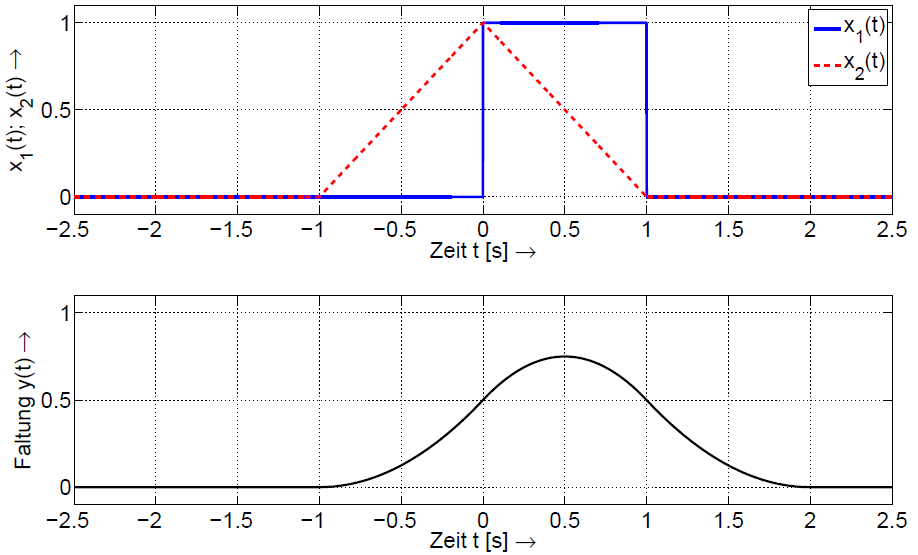
\includegraphics[width=0.8\textwidth]{Bilder/Faltung.png}
	\caption{Quelle: Skript SigSys}
\end{figure}
%
\subsubsection[Rechenregeln]{Rechenregeln}
	\begin{minipage}{0.33\textwidth}
		\textbf{Kommutativität}\\
		$f *(g * h)=(f * g) * h$
	\end{minipage}
%
	\begin{minipage}{0.33\textwidth}
		\textbf{Assoziativität}\\
		$f *(g * h)=(f * g) * h$
	\end{minipage}
%
	\begin{minipage}{0.33\textwidth}
		\textbf{Distributivität}\\
		$f *(g+h)=(f * g)+(f * h)$
	\end{minipage}\\
%
\subsubsection[Faltung mit der $\delta$-Funktion]{Faltung mit der $\delta$-Funktion}
\begin{minipage}{0.5\textwidth}
	$f(t) * \delta\left(t-t_{0}\right)=f\left(t-t_{0}\right)$
\end{minipage}\\
%

\subsection[Laplacetransformation]{Laplacetransformation}
Gegenüber j$\omega$ bei der Fourier-Transformation ist bei der Laplace-Transformation $s$ verallgemeinert zu $s=\sigma + j\omega$. Das bedeutet, dass die Fourier-Transformierte $F(j\omega)$ durch die Laplace-Transformation $F(s)$ ausgedrückt werden kann.
\begin{minipage}{0.35\textwidth}
	\begin{framed}
		\centering
		$f(t)\laplace F(s) = \int_{0}^{\infty}f(t)e^{-st}dt$
	\end{framed}
\end{minipage}
\begin{minipage}{0.13\textwidth}
	\fbox{\centering$s=\sigma+j\omega$}
\end{minipage}
\begin{minipage}{0.52\textwidth}
	$\left\lbrace
		\begin{array}{l}
			\sigma=0 \rightarrow$Amplitude bleibt gleich$\\
			\sigma> 0 \rightarrow$Amplitude explodiert für $0<t\rightarrow\infty\\
			\sigma< 0 \rightarrow$Amplitude klingt für $0<t\rightarrow\infty$ auf $0$ ab$
		\end{array}
	\right.$
\end{minipage}
\begin{itemize}
	\item Definitionsbereich nur für kausale Systeme $t\ge0$
	\item Wachstum kleiner als der von einer Exponentialfunktion
\end{itemize}
\subsubsection{Eigenschaften der Laplacetransformation}
\renewcommand{\arraystretch}{1.5}
\begin{tabular}{|l|l|}
	\hline Linearität	& $\alpha\cdot f(t) + \beta\cdot g(t) \laplace \alpha\cdot F(s) + \beta\cdot G(s)$\\
	\hline Ähnlichkeit / Streckung im Zeitbereich & $f(\alpha t) \; \laplace \; \frac{1}{\alpha}F(\frac{s}{\alpha})\quad (\alpha \in \mathbb{R})$\\
	\hline Faltung im Zeitbereich & $f(t) * g(t) \; \laplace \; G(s) \cdot F(s)$\\
	\hline 1te Ableitung im Zeitbereich & $\frac{\partial}{\partial t}f(t) \; \laplace \; sF(s) - f(0^{+})$\\
	\hline 2te Ableitung im Zeitbereich & $\frac{\partial^{2}}{\partial t^{2}}f(t) \; \laplace \; s^{2}F(s) - sf(0^{+}) - f'(0^{+})$\\
	\hline nte Ableitung im Zeitbereich & $\frac{\partial^{n}f(t)}{\partial t^{n}} \; \laplace \; s^{n}F(s) - s^{n-1}f(0^{+}) - s^{n-1}\frac{\partial f(0^{+})}{\partial t}- \ldots - s^{0}\frac{\partial^{n-1}f(0^{+})}{\partial t^{n-1}}$\\
	\hline Multiplikation mit t & $t \cdot f(t) \; \laplace \; \frac{-\partial F(s)}{\partial s}$\\
	\hline Ableitung im Frequenzbereich & $(-t)^{n} f(t) \; \laplace \; \frac{\partial^{n} F(s)}{(\partial s)^{n}}$\\
	\hline Verschiebung im Zeitbereich nach rechts & $\sigma(t-a)f(t - a) \; \laplace \; F(s)*e^{-as}$ \\
	\hline Verschiebung im Zeitbereich nach links & $\sigma(t-a)f(t + a) \; \laplace \; e^{as} \cdot [F(s) - \int\limits_0^{a} f(t) \cdot e^{-st} dt]$\\
	\hline Verschiebung im Frequenzbereich (Dämpfungssatz) & $f(t)e^{\pm\alpha t} \; \laplace \; F(s\mp\alpha)$ \\
	\hline Integration im Originalbereich (Sprungantwort)& $\int\limits_0^t f(u)du \; \laplace \; \frac{1}{s}\cdot F(s)$ \\
	\hline Anfangswert & $\lim_{t\rightarrow 0^+} f(t) = \lim_{s\rightarrow \infty} sF(s),\text{~wenn
	}  \lim_{t\rightarrow 0} f(t)\text{~existiert}.$ \\
	\hline Endwert & $\lim_{t\rightarrow \infty} f(t) = \lim_{s\rightarrow 0} sF(s),\text{~wenn
	}  \lim_{t\rightarrow \infty} f(t)\text{~existiert}.$ \\
	\hline
\end{tabular}
\renewcommand{\arraystretch}{1}
\subsubsection{Laplace-Tabelle}
\renewcommand{\arraystretch}{2}
\begin{minipage}{0.465\textwidth}
	\begin{center}
		\begin{tabular}{p{4cm}p{0.75cm}p{3cm}}
			$\sigma \left( t \right)$ & $\; \laplace \;$ & $\dfrac{1}{s}$ \\
			
			$\sigma \left( t \right) \cdot t$ & $\; \laplace \;$ & $\dfrac{1}{s^2}$\\
			
			$\sigma \left( t \right) \cdot t^2$ & $\; \laplace \;$ & $\dfrac{2}{s^3}$\\
			
			$\sigma \left( t \right) \cdot t^n$ & $\; \laplace \;$ & $\dfrac{n!}{s^{n+1}}$\\
			
			$\sigma \left( t \right) \cdot e^{\alpha t}$ & $\; \laplace \;$ &
			$\dfrac{1}{s-\alpha}$\\
			
			$\sigma \left( t \right) \cdot t \cdot e^{\alpha t}$ & $\; \laplace \;$ & $\dfrac{1}{( s - \alpha )^2}$\\
			
			$\sigma \left( t \right)\cdot t^2 \cdot e^{\alpha t}$ &
			$\; \laplace \;$ & $\dfrac{2}{{( s - \alpha )}^3}$\\
			
			$\sigma \left( t \right)\cdot t^n \cdot e^{ \alpha t}$ &
			$\; \laplace \;$ & $\dfrac{n!}{(s-\alpha)^{n+1}}$\\
			
			$\sigma \left( t \right)\cdot \dfrac { 1 - e ^ { - \alpha t } } { \alpha }$ & $\; \laplace \;$ & $\dfrac { 1 } { s ( s + \alpha ) }$\\
			
			$\sigma \left( t \right)\cdot \dfrac {e ^ { - \alpha t }+\alpha t -1 } { \alpha^2 }$ & $\; \laplace \;$ & $\dfrac { 1 } { s^2 ( s + \alpha ) }$\\
			
			$\sigma \left( t \right)\cdot \dfrac {1- e ^ { - \alpha t } - \alpha t e ^ {- \alpha t }}{ \alpha ^2 }$ & $\; \laplace \;$ & $\dfrac { 1 } { s ( s + \alpha )^2 }$\\		
		\end{tabular}
	\end{center}
\end{minipage}
\begin{minipage}{0.5\textwidth}
	\begin{center}
		\begin{tabular}{p{5cm}p{0.75cm}p{3cm}}
			
			$\delta \left( t \right)$ & $\; \laplace \;$ & $1\left( s \right)$ \\
			
			$\delta \left( t - \alpha \right)$ & $\; \laplace \;$ & $e^{- \alpha s}$\\
			
			$\sigma\left( t - \alpha \right)$ & $\; \laplace \;$ & $ \dfrac{1}{s} \cdot e^{- \alpha s}$\\
			
			$\sigma \left( t \right) \cdot \sin \left(\omega t \right)$ & $\; \laplace \;$ &
			$\dfrac{\omega}{s^2 + {\omega^2}}$\\
			
			$\sigma \left( t \right) \cdot \cos \left( \omega t \right)$ & $\; \laplace \;$ &
			$\dfrac{s}{ s^2 + \omega^2}$\\
			
			$\sigma \left( t \right) \cdot  e^{ \alpha t} \cdot \sin \left(\omega t \right)$ & $\; \laplace \;$ 
			& 	$\dfrac{\omega}{(s-a)^2 + {\omega^2}}$\\
			$\sigma \left( t \right) \cdot e^{ \alpha t} \cdot \cos \left( \omega t \right) $ & $\; \laplace \;$ &
			$\dfrac{s-a}{(s-a)^2 + \omega^2}$\\
			
			$\sigma \left( t \right)\cdot t \cdot \dfrac{\sin \left( \alpha t \right)} { 2 \alpha }$ & $\; \laplace \;$ & $\dfrac{s}{ \left(s^ {2}+ \alpha ^{2} \right)^{2}}$ \\
			
			$\sigma \left( t \right)\cdot \dfrac { e ^ { - \alpha t } - e ^ { - \beta t } } { \beta - \alpha }$ & $\; \laplace \;$ & $\dfrac { 1 } { ( s + \alpha ) ( s + \beta ) }$\\
			
			$\sigma \left( t \right)\cdot \dfrac {(\alpha - \beta) +\beta e ^ { - \alpha t } - \alpha e ^ { - \beta t } } { \alpha \beta (\alpha - \beta) }$ & $\; \laplace \;$ & $\dfrac { 1 } {s ( s + \alpha ) ( s + \beta ) }$\\
			
			$\sigma \left( t \right)\cdot \dfrac { e ^ { - \beta t } ( \alpha \cos ( \alpha t ) - \beta \sin ( \alpha t ) ) } { \alpha }$& $\; \laplace \;$ & $\dfrac { s } { ( s + \beta ) ^ { 2 } + \alpha ^ { 2 } }$\\
		\end{tabular}
	\end{center}
\end{minipage}
\renewcommand{\arraystretch}{1}
 %Nithu
	%Erst später
	%\newpage
	%\section{Funktionen mehrerer Variablen}
 
	
\end{document}